%\documentclass[a4paper,10pt]{article}
\documentclass[a4paper]{article}
%\usepackage[paper=a4paper, hmargin=0.5cm, bottom=0.5cm, top=0.5cm]{geometry}
\usepackage[latin1]{inputenc}
\usepackage[T1]{fontenc}
\usepackage[spanish]{babel}
\usepackage{xspace}
\usepackage{xargs}
\usepackage{ifthen}
\usepackage{listings}
\usepackage{aed2-symb,aed2-itef,aed2-tad,caratula}
\usepackage{xcolor}
\usepackage{listings}
\usepackage{soul}
\usepackage{tikz}
\usepackage{MnSymbol}

%Tikz library
\usetikzlibrary{positioning}
\usetikzlibrary{arrows}
\usetikzlibrary{graphs,graphs.standard,quotes}
\usetikzlibrary[topaths]

%lo agregue yo
\usepackage{graphicx}
\graphicspath{ {imagenes/} }
\usepackage{pgfplots}
\usepackage{tikz}

\usepackage[T1]{fontenc}
\usepackage{inconsolata}

\usepackage{color,soul}

\definecolor{pblue}{rgb}{0.13,0.13,1}
\definecolor{pgreen}{rgb}{0,0.5,0}
\definecolor{pred}{rgb}{0.9,0,0}
\definecolor{pgrey}{rgb}{0.46,0.45,0.48}

\usepackage{tabulary}

\usepackage{listings}
\lstset{language=Java,
  showspaces=false,
  showtabs=false,
  breaklines=true,
  showstringspaces=false,
  breakatwhitespace=true,
  commentstyle=\color{pgreen},
  keywordstyle=\color{pblue},
  stringstyle=\color{pred},
  basicstyle=\ttfamily,
  moredelim=[il][\textcolor{pgrey}]{$$},
  moredelim=[is][\textcolor{pgrey}]{\%\%}{\%\%}
}

\usepackage[latin1]{inputenc} 
\usepackage{multirow}

\newcommand{\moduloNombre}[1]{\textbf{#1}}
\newcommand{\bigO}{\mathcal{O}}
\newcommand{\complejidad}[2]{\hfill $#1 \bigO(#2)$}

\let\NombreFuncion=\textsc
\let\TipoVariable=\texttt
\let\ModificadorArgumento=\textbf
\newcommand{\res}{$res$\xspace}
\newcommand{\tab}{\hspace*{7mm}}

\newcommandx{\TipoFuncion}[3]{%
\NombreFuncion{#1}(#2) \ifx#3\empty\else $\to$ \res\,: \TipoVariable{#3}\fi%
}
\newcommand{\In}[2]{\ModificadorArgumento{in} \ensuremath{#1}\,: \TipoVariable{#2}\xspace}
\newcommand{\Out}[2]{\ModificadorArgumento{out} \ensuremath{#1}\,: \TipoVariable{#2}\xspace}
\newcommand{\Inout}[2]{\ModificadorArgumento{in/out} \ensuremath{#1}\,: \TipoVariable{#2}\xspace}
\newcommand{\Aplicar}[2]{\NombreFuncion{#1}(#2)}

\newlength{\IntFuncionLengthA}
\newlength{\IntFuncionLengthB}
\newlength{\IntFuncionLengthC}
%InterfazFuncion(nombre, argumentos, valor retorno, precondicion, postcondicion, complejidad, descripcion, aliasing)
\newcommandx{\InterfazFuncion}[9][4=true,6,7,8,9]{%
  \hangindent=\parindent
  \TipoFuncion{#1}{#2}{#3}\\%
  \textbf{Pre} $\equiv$ \{#4\}\\%
  \textbf{Post} $\equiv$ \{#5\}%
  \ifx#6\empty\else\\\textbf{Complejidad:} #6\fi%
  \ifx#7\empty\else\\\textbf{Descripci\'on:} #7\fi%
  \ifx#8\empty\else\\\textbf{Aliasing:} #8\fi%
  \ifx#9\empty\else\\\textbf{Requiere:} #9\fi%
}

\newenvironment{Interfaz}{%
  \parskip=2ex%
  \noindent\textbf{\Large Interfaz}%
  \par%
}{}

\newenvironment{Representacion}{%
  \vspace*{2ex}%
  \noindent\textbf{\Large Representaci\'on}%
  \vspace*{2ex}%
}{}

\newenvironment{Algoritmos}{%
  \vspace*{2ex}%
  \noindent\textbf{\Large Algoritmos}%
  \vspace*{2ex}%
}{}


\newcommand{\titlex}[1]{
  \vspace*{1ex}\par\noindent\textbf{\large #1}\par
}

\newenvironmentx{Estructura}[2][2={estr}]{%
  \par\vspace*{2ex}%
  \TipoVariable{#1} \textbf{se representa con} \TipoVariable{#2}%
  \par\vspace*{1ex}%
}{%
  \par\vspace*{2ex}%
}%

\newboolean{EstructuraHayItems}
\newlength{\lenTupla}
\newenvironmentx{Tupla}[1][1={estr}]{%
    \settowidth{\lenTupla}{\hspace*{3mm}donde \TipoVariable{#1} es \TipoVariable{tupla}$($}%
    \addtolength{\lenTupla}{\parindent}%
    \hspace*{3mm}donde \TipoVariable{#1} es \TipoVariable{tupla}$($%
    \begin{minipage}[t]{\linewidth-\lenTupla}%
    \setboolean{EstructuraHayItems}{false}%
}{%
    $)$%
    \end{minipage}
}

\newcommandx{\tupItem}[3][1={\ }]{%
    %\hspace*{3mm}%
    \ifthenelse{\boolean{EstructuraHayItems}}{%
        ,#1%
    }{}%
    \emph{#2}: \TipoVariable{#3}%
    \setboolean{EstructuraHayItems}{true}%
}

\newcommandx{\RepFc}[3][1={estr},2={e}]{%
  \tadOperacion{Rep}{#1}{bool}{}%
  \tadAxioma{Rep($#2$)}{#3}%
}%

\newcommandx{\Rep}[3][1={estr},2={e}]{%
  \tadOperacion{Rep}{#1}{bool}{}%
  \tadAxioma{Rep($#2$)}{true \ssi #3}%
}%

\newcommandx{\Abs}[5][1={estr},3={e}]{%
  \tadOperacion{Abs}{#1/#3}{#2}{Rep($#3$)}%
  \settominwidth{\hangindent}{Abs($#3$) \igobs #4: #2 $\mid$ }%
  \addtolength{\hangindent}{\parindent}%
  Abs($#3$) \igobs #4: #2 $\mid$ #5%
}%

\newcommandx{\AbsFc}[4][1={estr},3={e}]{%
  \tadOperacion{Abs}{#1/#3}{#2}{Rep($#3$)}%
  \tadAxioma{Abs($#3$)}{#4}%
}%

\usepackage{pdfpages}
% \lstset {
%     language=C++,
%     backgroundcolor=\color{black!5}, % set backgroundcolor
%     basicstyle=\footnotesize,% basic font setting
% }

\usepackage{xcolor,colortbl}
\definecolor{green}{rgb}{0.1,0.1,0.1}
% Enter this in the cell you wish to color a light grey.
% NB: the word 'gray' here denotes the grayscale color scheme, not the color grey. '0.9' denotes how dark the grey is.

\definecolor{pblue}{rgb}{0.13,0.13,1}
\definecolor{pgreen}{rgb}{0,0.5,0}
\definecolor{pred}{rgb}{0.9,0,0}
\definecolor{pgrey}{rgb}{0.46,0.45,0.48}
\usepackage{listings}
\lstset{language=Java,
  showspaces=false,
  showtabs=false,
  breaklines=true,
  showstringspaces=false,
  breakatwhitespace=true,
  commentstyle=\color{pgreen},
  keywordstyle=\color{pblue},
  stringstyle=\color{pred},
  basicstyle=\ttfamily,
  moredelim=[il][\textcolor{pgrey}]{$$},
  moredelim=[is][\textcolor{pgrey}]{\%\%}{\%\%}
}

\begin{document}

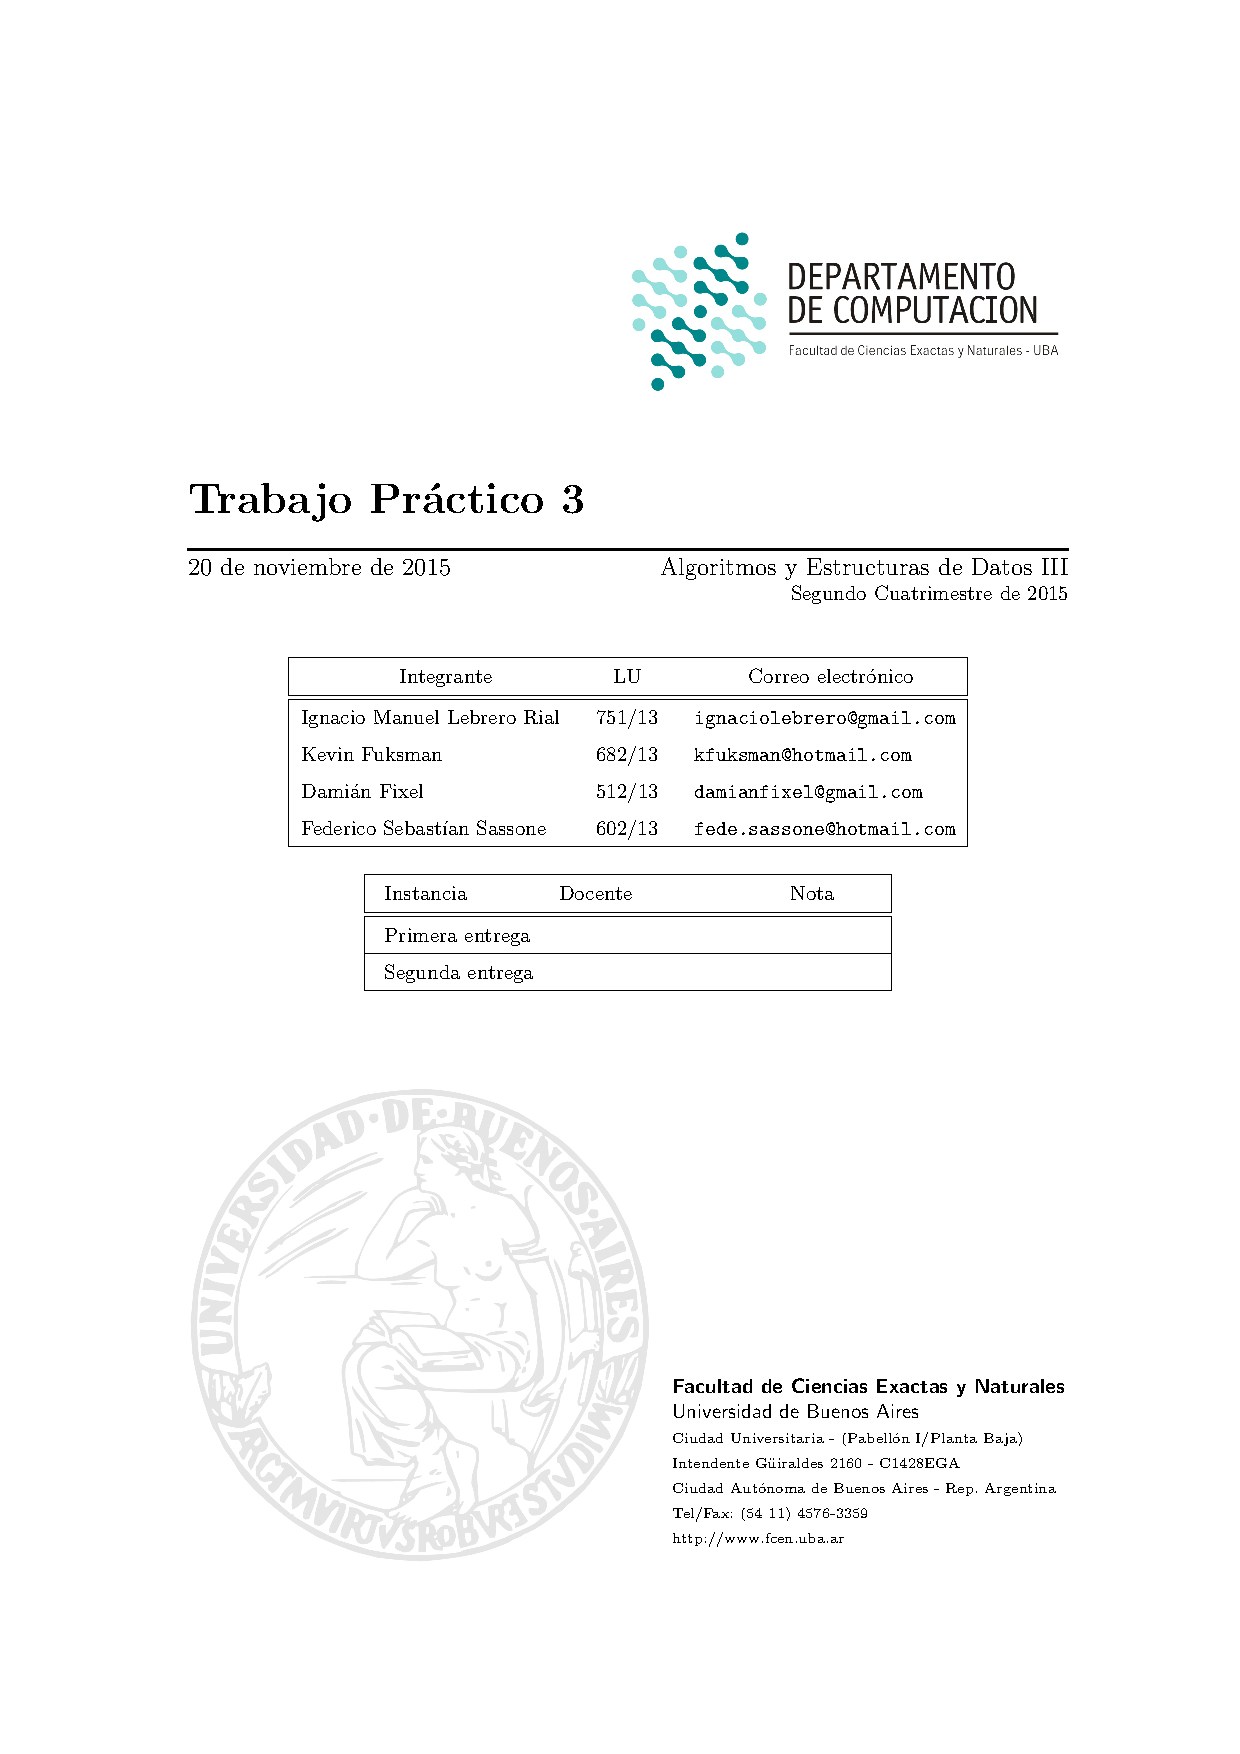
\includepdf{caratula}

% compilar 2 veces para actualizar las referencias
\tableofcontents

\pagebreak
\section{Ejercicio 1}
\subsection{Problema}
Dise\~nar e implementar un \textbf{algoritmo exacto} para el caso en el que cada materia tiene un
de 2 aulas posibles donde se podr\'a dictar. Este problema, donde cada v\'ertice tiene un m\'aximo de 2 colores disponibles se conoce como 2-List Coloring y tiene soluci\'on en tiempo polinomial.

\subsection{Explicacion y desarrollo del problema}     
Hay materias a las que se les pueden asignar un m\'aximo de dos aulas posibles donde dictarse y cumplen con una franja horaria determinada por mater\'ia.\\
Para este problema se nesecita saber si existe una organizaci\'on de aulas de manera que todas las materias puedan ser dictadas en sus respectivos horarios y de existir una soluci\'on encontrarla.
Para modelar el problema se define un grafo $G = (V,E)$ tal que para todo $v$ $\in$ $V$, $v$ representa una materia. y para todo par $(v,w)$ $\in$ $E$, este par existe si y solo si la interseccion de horarios de las materias $v$ y $w$ es no vacia. Por otro lado se definen los posibles colores que puede tener un nodo como las aulas a las que puede ser asignada la materia a la representa.\\

\vspace{5mm}
{\centering
\tikzset{main node/.style={circle,fill=white!20,draw,minimum size=1cm,inner sep=0pt},}
\begin{tikzpicture}
    %\begin{scope}[xshift=4cm]
    
    \node[main node] (1) {$V,B$};
    \node[main node] (2) [right = 1cm of 1] {$V,R$};
    
    \path[draw,thick]
    (1) edge node {} (2)
    ;
    %\end{scope}
\end{tikzpicture}

\begin{center}
    \caption{Dos nodos conectados con colores posibles $Verde$ y $Blanco$ y $Verde$ y $Rojo$ respectivamente.}
\end{center} \par
}
\vspace{5mm}

Luego, para encontrar una disposici\'on de aulas y materias de forma tal que no haya conflictos, si es posible, basta con encontrar un grafo con coloreo asociado a esa disposici\'on. En particular para este grafo se puede observar que, como maximo, cada materia tendr\'a asignadas dos posibles aulas, esto reduce el problema a uno en el que $G$ tendra un maximo de dos colores por nodo, este problema se denomina $2-List Coloring$.\\

Este puede ser reducido al problema de Satisficibilidad o $SAT$, que consiste en: sean $F_1,F_2,...,F_n$ formulas logicas de la forma $p_{i1} \lor p_{i2} \lor ... \lor p_{im}$ para $i \in [1,n]$. Se quiere saber si existe alguna combinacion de valores de verdad para todas las variables $p_{ij}$ tal que \\

{\centering
    $F_1 \land F_2 \land ... \land F_n$ \\
    $\equiv$ \\
    $(p_{11} \lor p_{12} \lor ... \lor p_{1m}) \land (p_{21} \lor p_{22} \lor ... \lor p_{2m}) \land ... \land (p_{n1} \lor p_{n2} \lor ... \lor p_{nm})$ \\ \par
}
\vspace{5mm}

sea verdadera. Mas en particular, como la cantidad de colores es a lo sumo dos, puede ser reducido a $2-SAT$ donde las formulas tienen a lo sumo dos literales, en este caso $m$ quedar\'ia acotado por dos.\\

Veamos como se reduce: cada nodo puede tener hasta dos colores, pero solo puede estar pintado de uno a la vez, para esto el nodo puede tener hasta dos estados: $p_1$ \'o $p_2$, con $p_1$ y $p_2$ los colores posibles respectivos. reescribiendo queda \\

{\centering
    $p_1 \lor p_2 \equiv (\neg p_1 \Rightarrow p_2) \land (\neg p_2 \Rightarrow p_1))$\\ \par
}
\vspace{5mm}

Asi podemos reescribir cada nodo en $2$ o $4$ nodos donde cada uno representara un color o la negacion del mismo y donde $u,v$ tiene un eje que sale de $u$ y va a $v$ si $u = \neg v$. 

\vspace{5mm}
    %ejemlo de los 4 nodos conectados
    \begin{center}
        \tikzset{main node/.style={circle,fill=white!20,draw,minimum size=1cm,inner sep=0pt},}
\begin{tikzpicture}
    %\begin{scope}[xshift=4cm]

    \node[main node] (1) {$V$};
    \node[main node] (2) [right = 1cm of 1] {$¬V$};
    \node[main node] (3) [above = 1cm of 1] {$F$};
    \node[main node] (4) [right = 1cm of 3] {$¬F$};
    ;
    
    \path[draw,thick]
    (1) edge node {} (2)
    (3) edge node {} (4)
    ;
    %\end{scope}
\end{tikzpicture}


        \caption{NodosPredicado}
    \end{center}
%TODO: agregar flechas
\vspace{5mm}
%TODO: explicar caso de 1 solo color

Al haber dos materias cuyos horarios tengan intersecci\'on no vacia y compartan algun color aplicamos la relacion previamene definida.

\vspace{5mm}
    %ejemplo de dos nodos materias conectando sus predicados
    \begin{center}
        \tikzset{main node/.style={circle,fill=white!20,draw,minimum size=1cm,inner sep=0pt},}



\begin{tikzpicture}
    %\begin{scope}[xshift=4cm]
    

    \node[main node] (1) {A$[V]$};
    \node[main node] (2) [red][above = 1cm of 1] {\textcolor{white}{A$[¬V]$}};
    \node[main node] (3) [red][above = 1cm of 2] {\textcolor{white}{A$[F]$}};
    \node[main node] (4) [above = 1cm of 3] {A$[¬F]$};
    
    
    \node[main node] (5) [right = 3cm of 1] {B$[F]$};
    \node[main node] (6) [red][right = 3cm of 2] {\textcolor{white}{B$[¬F]$}};
    \node[main node] (7) [red][right = 3cm of 3] {\textcolor{white}{B$[R]$}};
    \node[main node] (8) [right = 3cm of 4] {B$[¬R]$};
    
    
    
    \path[draw,thick]
        %intermedias
        
        %\chainin (4-5)
        (4) edge node {} (5)
        (6) edge node {} (3)
        
        %nodo1
        (2) edge node {} (1)
        (4) edge node {} (3)
        
        %nodo2
        (6) edge node {} (5)
        (8) edge node {} (7)
    ;
    %\end{scope}
\end{tikzpicture}
    \end{center}
\vspace{5mm}

de esta manera transformamos el grafo de materias orginal en un digrafo de predicados logicos con sus respectivas implicaciones. estas dan un coloreo parcial del grafo original ya que al implicar que colores deben valer da informacion sobre como pintar el grafo.\\

%ejemplo de predicados

A continuacion se necesita tomar todas estas componentes conexas para obtener un posible coloreo de un grafo y, haciendo uso de la transitividad del operador "$\Rightarrow$", ver que no se haya generado una contradiccion, esto es que $p$ y $\neg p$ pertenezcan a la misma componente conexa, lo que significaria que pintar de $p \Rightarrow \neg p$ y viceverza, con lo que no existiria un coloreo valido.

%ejemplo componente furtemente conexa

Para obtener las componentes se usa el algoritmo de kosaraju (explicado en clase), el cual devuelve las componentes en orden topologico, esto servira para obtener un coloreo valido en caso de que este exista.

Solo queda ver como formar un coloreo valido a partir de lo que las componentes obtenidas, para esto debemos ir formando constructivamente una sucesion de estados validos de manera que no lleguemos a una implicacion invalida, esto es haber asumido que un color $p$ es veradero en alguna componente (y como consecuencia, pintar el nodo correspondiente de ese color) y al estar agregando colores verdaderos en otra componente llegar a que el nodo previamente coloreado deba ser $\neg p$. En ese caso no ser\'ia coloreo valido. \\

Para evitar estas contradicciones usamos la siguiente t\'ecnica de coloreo: Como las componentes vienen dadas en orden topologico, definimos que una componente tiene valor $true$ si para pintar se utilizan sus nodos $p$ y es $false$ si se usan los nodos $\neg p$.

%dibujo componente inicial con todos false

Se empieza colocando la primera componente del orden topologico en false y pintano todos nodos, recordemos que a esta altura ya esta chequeado que no hay contradicciones en las componentes por separado con lo que se puede pintar tranquilamente. Luego pasamos a las siguientes componentes, al estar en orden topologico estas tienen algun nodo que esta conectado con la primera de manera $u \Rightarrow v$ con $u$ en el primero nodo y $v$ en el actual. como pintamos a todos los nodos de la primer componente en false, seguiremos pintando false. Esto es valido ya que el coloreo de estos nodos se puede decir que esta $implicado$ por los colores de la primer componente ya que hay algun eje que sale de la primera y va hacia la actual, y como $false \Rightarrow false$ es $true$ este sigue siendo un coloreo valido. \\

%dibujo de nodos componente false implica false

Puede llegar el momento en el que aparece una contradiccion, de pasar esto simnplemente se invierte el valor de verdad de la componente y pasa a ser $true$, esto es valido ya que era implicada por una componente $false$ y $false \Rightarrow true \equiv true$ con lo que sigue siendo un coloreo valido. \\

%dibujo de nodos componente false implica true

A partir de ese momento todas las componentes que sean implicadas de esta deben ser $true$, de no llegar a serlo (que hubiese una contradiccion) no habria coloreo posible para el grafo, esto se puede ver porque habr\'ia que invertir el valor de verdad de la componente a $false$ pero el nodo que la implicaba era $true$ y $true \Rightarrow false \equiv false$ con lo que quedaria un coloreo invalido del grafo por generar una contradiccion.   

\pagebreak

\subsection{Pseudo-C\'odigo}

\begin{verbatim}
kosaraju (GrafoPredicados grafo)
    boolean [] usado = new boolean[grafo.sizeEstados()];  
    ArrayList< NodoEstado > orden = new ArrayList<NodoEstado>() 
    ArrayList< Componente > componentes = new ArrayList< Componente >() 
    
    FOR i = 0 WHILE i < usado.length STEP i++
        IF !usado[i] THEN
            dfs(grafo.getNodosEstado(), usado, orden, i);
        ENDIF
    ENDFOR
    ArrayList<NodoEstado> grafoInvertido = grafo.grafoInvertido(); 
    Collections.reverse(orden); 
    Arrays.fill(usado, false); 
    
    FOREACH NodoEstado m IN orden 
        IF !usado[ m.getId() ] THEN
            ArrayList<NodoEstado> componenteActual = new ArrayList<NodoEstado>(); 
            
            dfs(grafoInvertido, usado, componenteActual, m.getId());
            FOREACH NodoEstado n IN componenteActual 
                n.setCC( componentes.size() ); 
            ENDFOR
            componentes.add(new Componente(componenteActual, componentes.size())); 
        ENDIF
    ENDFOR
    RETURN componentes;

dfs (ArrayList< NodoEstado > g, boolean[] usado, List< NodoEstado > m, int i)
    NodoEstado actual = g.get(i); 
    usado[ actual.getId() ] = true; 
    
    FOREACH NodoEstado vecino IN actual.getAdyacentes()
        IF (!usado[ vecino.getId() ])
            dfs(g, usado, m, vecino.getId());
        ENDIF
    ENDFOR
    m.add(actual);

tieneSolucion(ArrayList< Componente > componentes)
    FOREACH Componente c IN componentes
        c.valordeVerdad();    
    ENDFOR
    RETURN checkThrtuthValues(componentes);

checkThrtuthValues(ArrayList< Componente > componentes)
    boolean result = true;
    FOREACH Componente c IN componentes
        result = result && !c.valorDeVerdad;
    RETURN result;

armarColoreo(ArrayList<Componente> componentes)
    ArrayList<Color> solucion = new ArrayList<Color>();
    boolean usados[] = new boolean[cantMaterias];
    int ocupados = 0;
    
    WHILE ocupados < cantMaterias 
        FOREACH Componente c IN componentes 
            FOREACH NodoEstado n IN c.nodos 
                IF n.getNegado() && !usados[n.getPadreId()] THEN
                    Color colorActual = new Color(n.getColor(), n.getPadreId());
                    
                    solucion.add(colorActual);
                    usados[n.getPadreId()] = true;
                    ocupados++;
                ENDIF
            ENDFOR
        ENDFOR
    ENDWHILE
    RETURN solucion;

armarGrafoDeComponentesConexas (ArrayList<Componente> componentes)
    FOREACH Componente c in componentes 
        FOREACH NodoEstado actual in c.nodos 
            FOREACH NodoEstado adyacente in actual.getAdyacentes() 
                IF adyacente.getIdCC() != actual.getIdCC()
                    c.addVecino(componentes.get(adyacente.getIdCC()));
                ENDIF
            ENDFOR
        ENDFOR
    ENDFOR

solve (GrafoPredicados grafo)
    grafo.generarGrafoDeEstados();
    ArrayList< Componente > componentesConexas = kosaraju(grafo);
    
    IF tieneSolucion(componentesConexas)
        armarGrafoDeComponentesConexas(componentesConexas);
        ArrayList<Color> sol = armarColoreo(componentesConexas);
        return sol;
    ELSE
        return null;
    ENDIF
\end{verbatim}
\pagebreak

\subsection{Justificaci\'on y Complejidad}
$Observacion:$ N = cantidad de nodos del grafo de materias,\\ M = cantidad de ejes del grafo de materias, NP = nactidad de nodos del grafo de predicados, MP = cantidad de ejes del grafo de predicados. \\

El algoritmo consta de $5$ partes:

\begin{itemize}
    \item Armar el grafo de predicados (1)
    \item Kosaraju (2)
    \item Chequear contradicciones (3)
    \item Conectar las componentes fuertemente conexas (4)
    \item Armar un coloreo (5)
\end{itemize}

Analicemos un poco el pseudocodigo para ver que pinta tendra la complejidad.

\begin{verbatim}
solve(GrafoPredicados grafo)
    grafo.generarGrafoDePredicados(); (1)
    ArrayList< Componente > componentesConexas = kosaraju(grafo); (2)
    IF (tieneSolucion(componentesConexas)){ (3)
        armarGrafoDeComponentesConexas(componentesConexas); (4)
        ArrayList<Color> sol = armarColoreo(componentesConexas); (5)
		
        RETURN sol;
    ELSE
        RETURN null;
    ENDIF
\end{verbatim}\\

El algoritmo tendra complejidad en peor caso $\theta((1) + (2) + (3) + (4) + (5))$. A continuacion se analizara cada parte en detalle. \\

\subsubsection {Grafo de Predicados}

Al iniciar el algoritmo se recibe un objeto $GrafoDePredicados$ el cual solo contiene el grafo de materias, en este momento se genera el grafo de predicacdos con sus conexiones respectivas.

\begin{verbatim}
    generarGrafoDePredicados() {
        grafoEstados = new ArrayList<NodoPredicado>(); O(1)
		
        for (NodoMateria m : grafoMateria) { O(N)
            generarNodosPredicado(m); O(1)
        }

        for (Conexion c : conexiones) { O(M)
            conectarEstados(c); O(1)
        }
    }
\end{verbatim}

veamos ahora los m\'etodos que son llamados internamente.\\

\begin{verbatim}
generarNodosPredicado(NodoMateria m)
    IF m.getColores().size() > 0
        ArrayList<NodoPredicado> estadosActuales;  O(1)
        int id, idPadre, color[], cantidadColores; O(1)
		
        id 		= grafoEstados.size();             O(1)
        color 	= new int[2];                      O(1)
        idPadre = m.getId();                       O(1)
        cantidadColores = m.getColores().size();   O(1)
		
        FOR i = 0 WHILE i < cantidadColores STEP ++i O(1) <- acotado por 2
            color[i] = m.getColor(i); O( 1 )
        ENDFOR
		
        estadosActuales = crearNodos(id, idPadre, color, cantidadColores); O (1)
        conectarEstadosInternos( estadosActuales ); O (1)

        FOR NodoPredicado actual : estadosActuales O (1) <- acotado por 4
            grafoEstados.add( actual ); O (1)
        ENDFOR
        
        m.addEstados( estadosActuales ); O (1) <- acotado por 4
    ENDIF
\end{verbatim}

Finalmente la complejidad queda O( N + M )

\subsubsection {Kosaraju}
Se dio en clase, su complejidad es O ( NP + MP )

\subsubsection {contradicciones}

\begin{verbatim}
tieneSolucion(ArrayList< Componente > componentes)
    FOR Componente c : componentes O(NP)
        c.valordeVerdad(); O(MP)
    ENDFOR
	
    return checkThruthValues(componentes); O(NP)
\end{verbatim}
		
La funcion valor de verdad recorre linealmente los nodos de la componente fuertemente conexa y checkTruthValues reviza que no ninguna componente sea verdadera (que exista una contradiccion). La complejidad queda O (NP + MP).

\pagebreak
\subsubsection {Conectar componentes}
\begin{verbatim}
armarGrafoDeComponentesConexas(ArrayList<Componente> componentes)
    FOR (Componente c : componentes)
        FOR (NodoEstado actual : c.nodos)
            FOR (NodoEstado adyacente : actual.getAdyacentes())
                IF (adyacente.getIdCC() != actual.getIdCC())
                    Componente vecino = componentes.get(adyacente.getIdCC()); 
                    c.setPadre(vecino);

el algoritmo recorre todas las conexiones que hay, queda O(MP).
\end{verbatim}

\subsubsection {Armar coloreo}

\begin{verbatim}
armarColoreo(ArrayList<Componente> componentes) {
    Color [] solucion = new Color[cantMaterias];
    int usados[] = new int[cantMaterias];
    boolean pintadaActual;
    int ocupados = 0;
    
    while (ocupados < cantMaterias) {
        for (Componente c : componentes) {

            //valor de verdad actual
            if (c.hasPadre()) {
                if (c.getValorVerdadPadre()) {
                    pintadaActual = true;
                } else {
                    pintadaActual = false;
                }
            } else {
                pintadaActual = false;
            }
            
            //checkeo por contradicciones contra el coloreo armado
            for (NodoPredicado n : c.nodos) {
                if (usados[n.getPadreId()] == -1) {
                    if (n.getColor() == solucion[n.getPadreId()].getColor() && n.getNegado()) {
                        if (pintadaActual = true) { 
                            return null;
                        } else {
                            pintadaActual = true;
                            c.setValorDeVerdad(true);
                        }
                    }
                } else {
                    if (usados[n.getPadreId()] == 1) {
                        if (n.getColor() == solucion[n.getPadreId()].getColor() && !n.getNegado()) {
                            if (pintadaActual = true) { 
                                return null;
                            } else {
                                pintadaActual = true;
                                c.setValorDeVerdad(true);
                            }
                        }
                    }
                }
            }
            
            //armo el coloreo parcial
            for (NodoPredicado n : c.nodos) {
                if (!n.getNegado() == pintadaActual) {
                    if (usados[n.getPadreId()] == 0) {
                        Color colorActual = new Color(n.getColor(), n.getPadreId());
                        
                        solucion[n.getPadreId()] = colorActual;
                        
                        if (n.getNegado()) {
                            usados[n.getPadreId()] = -1;
                        } else {
                            usados[n.getPadreId()] = 1;
                        }
                        
                        ocupados++;
                    }
                }
            }
        }
    }
    
    return solucion;
}
    \end{verbatim}
    
    Este algoritmo consta de 3 partes, la primera reviza cual es el valor de verdad de la componente padre. Recordemos que las componentes vienen dadas en orden topologico, y como se recorren linealmente se recorrera por niveles de este orden, la primera parte que reviza el valor de verdad solo hace comparaciones por lo que es constante, la segunda parte reviza todos los nodos de la componente para revizar que no haya contradicciones con respecto al coloreo que se venia armando, esto cuesta O(NP). la ultima parte arma efectivamente el coloreo, para esto se mueve por todos los nodosPredicadocon lo que tiene costo O(MP) y como se recorren todas las componentes en total queda O (NP + MP).
    
\pagebreak    
\subsubsection{Conclusion}

    Con lo que vimos hasta ahora podemos completar las incognitas que venian hasta ahora y queda: \\
    \begin{itemize}
        \item N + M (1)
        \item NP + MP (2)
        \item NP (3)
        \item MP (4)
        \item NP + MP (5)
    \end{itemize}
    
    Reescribiendo: \\
    
    {\centering
        \vspace{5mm}
        $O(N + M + NP + NP + MP + NP + MP + MP)$ \\
        \vspace{5mm}
        $O(N + M + NP + MP)$\\
        \vspace{5mm}
        \par
    }
    
    Como por cada nodoMateria se crean al menos dos nodosPredicados, la cantidad de estos va a ser mas grande, luego $N < NP$ y se puede acotar superiormente, con esto queda: \\
    
    {\centering
        \vspace{5mm}
        $O(N + M + NP + MP)$\\
        \vspace{5mm}
        $O(NP + MP + M)$ \\
        \vspace{5mm}
        \par
    }
\subsection{Correctitud}
La correctitud del algoritmo de kosaraju la vimos durante las clases por ende no es necesario demostrarla. Por otra parte, por la manera en la que definimos nuestras aristas, A es vecino de B si y solo si a=>b. De esta manera, todos los elementos que se encuentren en la componente fuertemente conexa, por la definicion de la misma, tienen un camino dirigido entre ellos.\\
Como la implicacion es transitiva, el tener un camino dirigido entre ellos significa que mediante una serie de implicaciones puedo llegar de una a la otra y viceversa, es decir que se implican mutuamente.\\
De esta manera si un nodo que representa " el nodo A debe pintarse de F", implica que "el nodo A NO debe pintarse de F" y viceversa, llegamos a una contradiccion y no existe coloreo posible.\\
Notemos que es independiente del color ya que al ser una serie de implicaciones, todo se reduce a encontrar que $p \leftrightarrow \neg p$

Solo queda probar que el coloreo que se forma es correcto, esto ya fue explicado en la seccion 1.2. 

\pagebreak

\subsection{Experimentaci\'on}
%moviendo nodos ejes estaticos
Previamente a analizar la performance del algoritmo veamos un poco su complejidad: O(NP + MP + M), como M y MP estan relacionadas, los experimentos van a ser en base a M y como NP y N (ver 1.4 para mas informacion) tambien estan relacionados, nos basaremos en N.\\
Veamos c\'omo var\'ian los tiempos de ejecuci\'on.

\subsubsection{Analisis sobre M}

Para el primer experimento simplemente mantuvimos N constante y aumentamos progresivamente M.
%nodos estaticos moviendo ejes
\begin{figure}[h!]
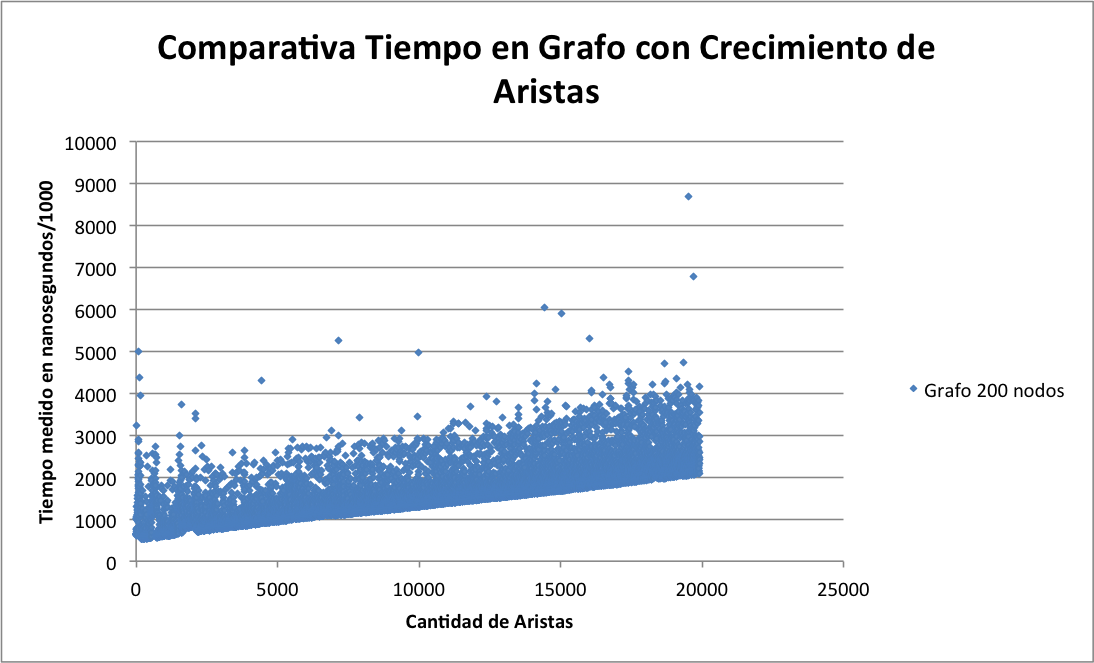
\includegraphics[width=140mm]{ejercicio1/ej1-grafo200-crecimientoaristas.png}
\centering 
\caption{Comparacion Tiempos de ejecucion - Cantiad de vertices fija, aristas variables}
\label{overflow3}
\end{figure}

Se puede ver que los tiempos aumentan linealmente a medida que la cantidad de aristas crece, esto se debe a que la creacion del grafo de predicados y la cantidad de elementos de las componentes conexas dependen fuertemente de N y M solo modifica la cantidad de conexiones que se crearan. \\

\pagebreak
\subsubsection{Analisis sobre N}

A continuaci\'on veamos que pasa cuando hacemos que M crezca de forma constante y aumentamos progresivamente N.\\
Los tiempos son en general mucho mayores y crecen m\'as r\'apido. Esto se debe nuevamente a que las operaciones sobre grafo de predicados y componentes conexas est\'an relacionadas con N y al aumentarlo, \'estas aumentan sus tiempos de ejecuci\'on. 

\begin{figure}[h!]
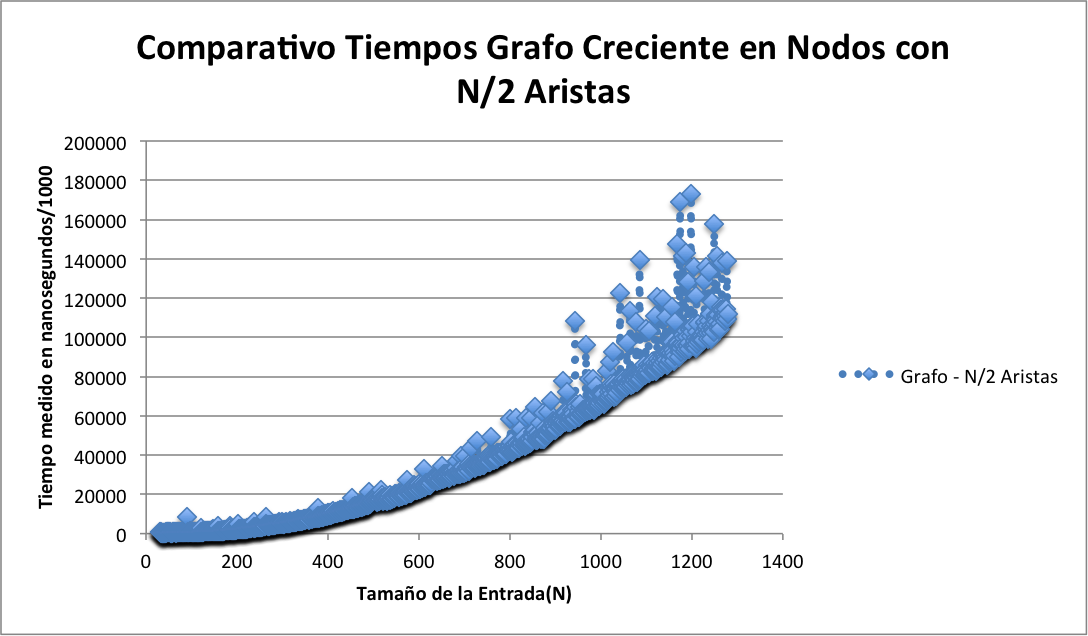
\includegraphics[width=140mm]{ejercicio1/ej1-grafo-nodosCreciente.png}
\centering
\caption{Comparacion Tiempos de ejecucion - Cantiad de aristas fija, nodos variables}
\label{overflow3}
\end{figure}

\pagebreak
\subsubsection{Analisis sobre Nodos y Colores}

Tuvimos la hip\'otesis de que un grafo de 50 nodos con 2 colores disponibles se iba a comportar igual que uno de 100 nodos con 1 color disponible. Asumimos que esto iba a ser as\'i por la cantidad de NodosPredicado que se crear\'ian en funci\'on de colores disponibles multiplicado por N, eso hubiera creado 200 NP en ambos grafos y los tiempos tendr\'ian que haberse parecido. Asumiamos que esto iba a ser una regla general.\\

Cuando hicimos el test nos dimos cuenta que est\'abamos equivocados en asumir que las conexiones iban a ser iguales en ambos grafos. Sin embargo llegamos a un gr\'afico que nos muestra el corportamiento lineal en ambas instancias.


\begin{figure}[h!]
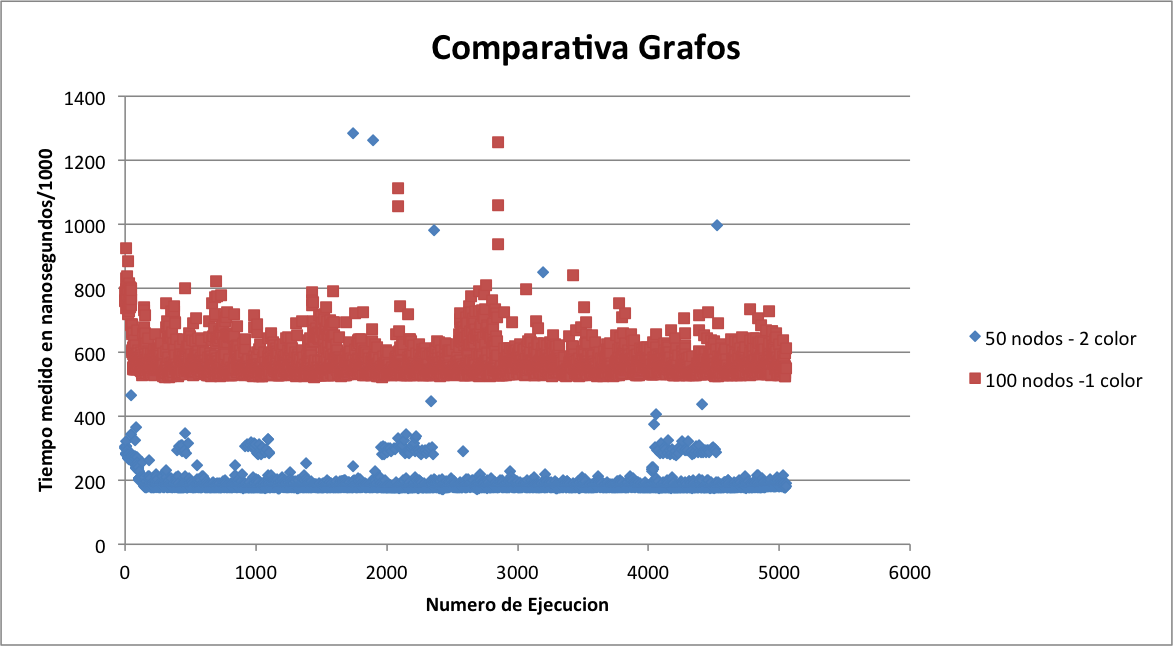
\includegraphics[width=140mm]{ejercicio1/ej1-grafo-relacionado.png}
\centering
\caption{Analisis sobre Nodos y Colores}
\label{overflow3}
\end{figure}

\pagebreak
\subsubsection{Generador de grafos}
Para generar nuestros grafos pseudo-aleatorios utilizamos el siguiente m\'etodo:\\
De antemano sabemos nuestros $N$ y $M$, tenemos un Array de nodos $[n_1,n_1,...,n_n]$,  comenzando desde $n_1$ buscamos el siguiente nodo $n_i$ con el que no tenga conexi\'on. Lanzamos una moneda cargada con una probabilidad, si da cara, conectamos el primer $n_1$ con nuestro $n_i$ y a $n_i$ con $n_1$. Repetimos hasta tener M conexiones o probar conectar $n_1$ con $n_n$, luego repetimos probando conexiones de $n_2$ y as\'i sucesivamente.

Los tiempos que figuran en el gr\'afico se deben a que al tener una probabilidad alta, las conexiones se hacen mucho m\'as rapido y esto trae como consecuencia que el grafo que se arma tenga componentes conexas m\'as grandes y que contienen nodos con id's m\'as bajas (Una alternativa para que las id's est\'en bien distribuidas era randomizar el orden de los nodos en el Arreglo, pero no lo tuvimos en cuenta).\\

Al variar la probabilidad vemos que con 75 se forman componentes m\'as pequenias y esto hace que el tiempo de  ejecuci\'on en grafos formados con esta probabilidad sea m\'as grande.

\begin{figure}[h!]
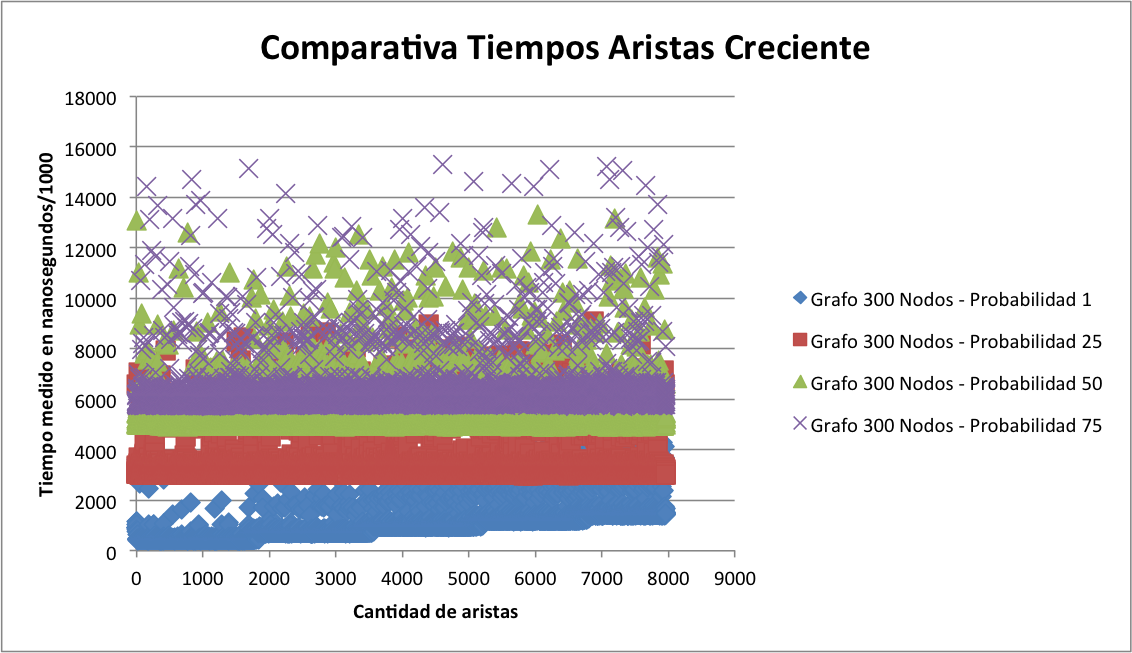
\includegraphics[width=140mm]{ejercicio1/ej1-grafo-aristasCreciente.png}
\centering
\caption{Tiempos de ejecuci\'on en grafos generados de distintas formas.}
\label{overflow3}
\end{figure}


\pagebreak
\pagebreak
\section{Ejercicio 2}
\subsection{Problema}
Dise\~nar e implementar un \textbf{algoritmo exacto} para List Coloring y desarrollar los siguientes puntos:\\

a) Explicar detalladamente el algoritmo implementado. Elaborar podas y estrategias que permitan mejorar los tiempos de ejecuci\'on. En los casos en los que el backtracking reduzca el problema a 2-List Coloring utilizar el algoritmo del item anterior como caso base.\\

b) Calcular el orden de complejidad temporal de peor caso del algoritmo.\\

c) Realizar una experimentaci\'on que permita observar los tiempos de ejecuci\'on del algoritmo en funci\'on del tama\~no de entrada y de las podas y/o estrategias implementadas.\\

\subsection{Explicaci\'on y desarrollo del problema}
Como vimos en clase, no se conoce ningun algortimo de orden polinomial para resolver este problema. Si bien no podremos mejorar la cota exponencial del algoritmo, nuestro objetivo estara en realizar un backtracking inteligente y distintas podas que ayuden a recortar el arbol de recursion y por ende achicar los tiempos de ejecucion. 

Recordemos que.. Backtracking(subsoluci\'on $s$):
\begin{itemize}
\item Si $s$ es invalido $\Rightarrow$ Falso
\item Si es $s$ valido $\Rightarrow$ res $<-s$ y Terminar
\item Si no, elegir una decicion D que falte tomar y para cada posible eleccion E de D, Backtracking($s+e$)
\end{itemize}
A este esquema la agregaremos dos tipos de podas. Una poda es una manera mas de saber cuando estamos en una subsolucion invalida.\\
La primera consiste en chequear si dada una materia A, pintada del color C, existe algun vecino tal que su unico color disponible es C. En ese caso sabemos que tendremos un conflicto ya que no podemos tener dos vecinos pintados del mismo color. Al encontrarnos con un conflictos, es en vano seguir por esa rama del backtracking por lo que decimos que el resultado de ir por ese lado es false y volvemos la recursion hacia atras.\\
La segunda poda es un poco mas compleja. Esta consiste en fijarse si existe un color disponible para mi materia tal que ese color no este diponible para ningun vecino. De esta manera, sabremos que esa materia puede pintarse exactamente de ese color y que no tendra ningun conflicto con sus vecinos (ya que como dijimos recien, ningun vecino tiene ese color). La implementacion va de la siguiente manera: Sea N la materia donde nos encontramos, preguntaremos si #(colores(N)) es mayor a #(colores(N)\ $\cap$ (vecinos(N)).\\
Esto quiere decir que existe un color K en N tal que no esta en ninguno de sus vecinos por ende puedo pintar automaticamente el nodo de color K.

%!% = Linea demasiado javaStyle para mi. Damian . tenias que escapear el "\cap"
\subsection{Pseudo-C\'odigo}
\begin{verbatim}


solverWithBacktrack()
    ArrayList<NodoMateria> nodos = new ArrayList<NodoMateria>();%!%
    ejercicio1 = new Ejercicio1(grafo.size());%!%
    FOREACH Materias(grafo) AS nodoMateria
        IF #ColoresPosibles(nodoMateria) > 2 THEN
            Agregar(nodoMateria, nodos)
         ELSE 
            FOR color desde 0 hasta ColoresPosibles(nodoMateria)
                Setearcolor(color,nodoMateria)
                ENDFOR
        ENDIF
    ENDFOR
    IF VACIO?(nodos) THEN
        RES = (solucion = ejercicio1.solve(grafo)) != NULL)%!%
    ELSE
        RES = backTrack(nodos);            
    ENDIF

backTrack(ArrayList<NodoMateria> materiasColores){
    NodoMateria materia = materiasColores.get(0)%!%
    materiasColores.remove(0);%!%
    bool solucion = false
    int i = 0
    
    IF poda2(materia) != -1 THEN
        materia.setColor(materia.getColores().get(i)); %!%
        if (backTrack(materiasColores))
            RES = true
        ENDIF
    ELSE 
            WHILE (i < #Colores(materia) || ! solucion)
                materia.setColor(materia.getColores().get(i)); %!%
                IF (poda1(materia,materia.getColores().get(i)))%!%
                    if #MateriasColores == 0 THEN
                        IF ejercicio1.solve() THEN 
                            RES = true
                        ELSE 
                            IF backTrack(materiasColores) THEN
                            RES = true
                            ENDIF
                        ENDIF        
                    ENDIF
                ENDIF
            ENDWHILE
    ENDIF
    RES = ejercicio1.solve
}
    
boolean poda1(NodoMateria materia, int color){
    FOREACH vecino(materia) AS materiaVecina
        IF #(Colores(materiaVecina)) == 1 && color PERTENECEA Colores(materiaVecina) THEN
            RES = false
        ENDIF
    ENDFOR
    
    RES = true
}
    
Integer poda2(NodoMateria materia){
    ArrayList<Integer> coloresPosibles = new ArrayList<Integer>(materia.getColores());%!%
    ArrayList<Integer> coloresVecinos  = new ArrayList<Integer>();%!%

    FOREACH Vecinos(materia) AS materiaVecina
        AgregarTodos(colores(materiaVecina), coloresVecinos)
    ENDFOREACH
    
    coloresPosibles.retainAll(coloresVecinos);%!%
    IF #coloresPosibles == #Colores(materia)
        RES = -1
        ELSE 
        FOR i desde 0 hasta #(Colores(materia)) 
            IF (!coloresPosibles.contains(materia.getColores().get(i)))%!%
                RES = materia.getColores().get(i);%!%
            ENDIF
        ENDFOR
    ENDIF
    
    RES = -1
}

solverWithBacktrack()
    nodos <- lista<Nodos>
    ejercicio1 <- InstanciaEj1(tamaño(grafo))
    
    FOREACH materias(grafo) AS  nodoMateria
        IF coloresPosibles(nodoMateria) > 2 THEN
            agregar(nodos,nodoMateria)
        ELSE
            FOREACH coloresPosibles(nodoMateria) AS color
                nodoMateria.setColor(color)
            ENDFOREACH
        ENDIF
    ENDFOREACH

    IF nodos.isEmpty() THEN
        DEVOLVER ejercicio1.solve(grafo)
    ELSE
        DEVOLVER backTrack(nodos)
    ENDIF

private boolean backTrack(ArrayList<NodoMateria> materiasColores){
    NodoMateria materia = desencolar(materiasColores)
    boolean tieneSolucion = false;
    int i = 0;
    IF poda2(materia) != -1 THEN
    materia.setColor(materia.getColores().get(i)); // Seteo el color de backtrack
    IF tamano(materiasColores) == 0 THEN
        IF ((solucion = ejercicio1.solve(grafo)) != null){
            DEVOLVER true;
        ENDIF
    ELSE
        IF backTrack(materiasColores)
            DEVOLVER true
        ENDIF
    ENDIF
    materia.clearColors()
    ELSE
        WHILE i < coloresPosibles(materia) ^ !tieneSolucion DO
    
            materia.setColor(materia.getColorPosible(i))
    
            IF (poda1(materia,materia.getColorPosible(i))){
                IF ((solucion = ejercicio1.solve(grafo)) != null){
                    DEVOLVER true;
                ENDIF
            ELSE
                IF backTrack(materiasColores)
                    DEVOLVER true
                ENDIF
            ENDIF
            i++;
            materia.clearColors();
            ENDIF
        ENDWHILE
    ENDIF
    materiasColores.add(0,materia);
    DEVOLVER false

\end{verbatim}
\pagebreak
\subsection{Justificaci\'on y Complejidad}
Como explicamos antes, no se conocen algoritmos en orden polinomial para resolver el problema por lo que nuestro algoritmo tiene una complejidad exponencial. Esta viene dada por el backtracking, el hecho de que explore todas las posibles combinaciones de colores que pueden tener los nodos da que la cantidad es $#colores(n_1) * #colores(n_2) * #colores(n_3) * .. * #colores(n_m)$ acotando la cantidad de colores por el mas grande queda $maxcolores * maxcolores * maxcolores * .. * maxcolores = maxcolores^{maxcolores}$.

\subsection{Correctitud}
Al explorar todas las posibles soluciones eventualmente encontrara una.

\subsection{Tests y Performance}
Vamos a separar nuestro analisis en dos partes. Por un lado queremos chequear si nuestras podas, independientemente de si mejoran o no en los tiempos de ejecucion, son efectivas en cuanto a la cantidad de subsoluciones que descarta. Cada vez que  nuestra poda resulte verdadera, sabremos que esa subsolucion analizada no es una subsolucion valida, por ende cortara la ejecucion y volvera hacia arriba en la recursion.  \\ 
El objetivo es ver como varia nuestra poda segun la dispersion que tengan los colores de cada nodo.\\ 
\begin{figure}[h!]
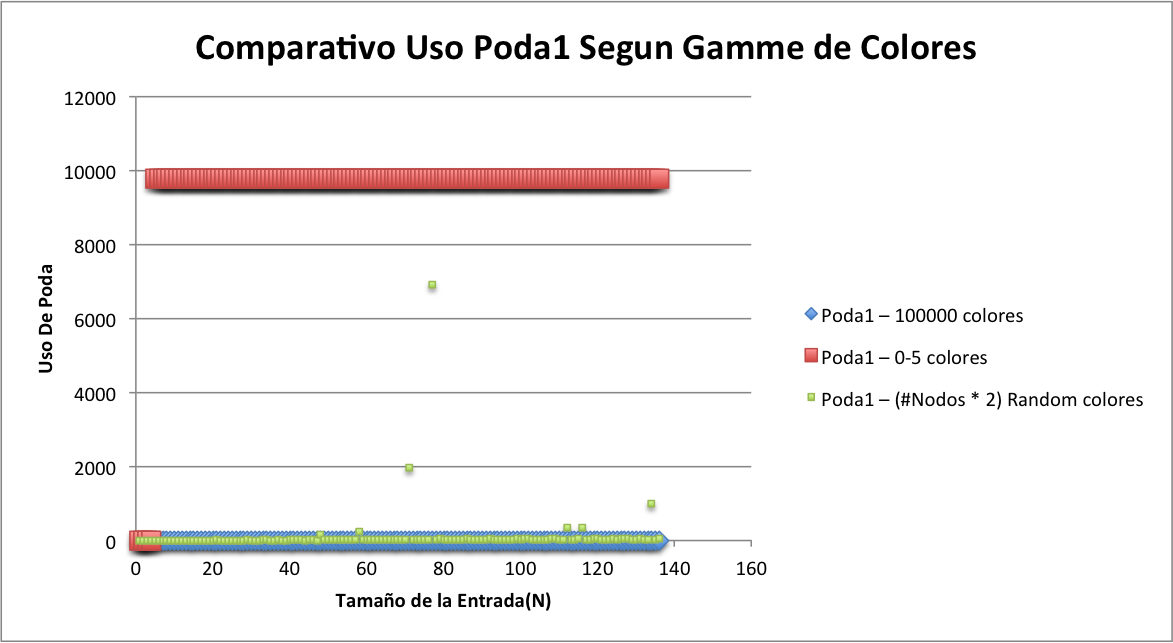
\includegraphics[width=140mm]{ejercicio2/ej2-comparativo-poda1-gammacolores.png}
\centering
\caption{Comparacion Uso de poda1 segun cantidad de colores posibles por nodo}
\label{overflow3}
\end{figure}\\
\pagebreak
Como podemos apreciar en el grafico, es muy claro que la poda1 solo sucede cuando la dispersion de colores es muy baja. Que quiere decir esto? Si nosotros tenemos muchos colores para elegir (por ejemplo un millon), es poco probable que tengamos un vecino que tenga un solo color disponible y que ademas sea el mismo en el cual estoy seteando el backtrack. Si la dispersion es baja, es mucho mas probable que nos encontremos con un color invalido(que ese color sea unico para algun vecino).\\
La conclusion que sacamos en que la poda1 se utiliza mucho siempre y cuando no tengamos una dispersion de colores muy grande.\\


\begin{figure}[h!]
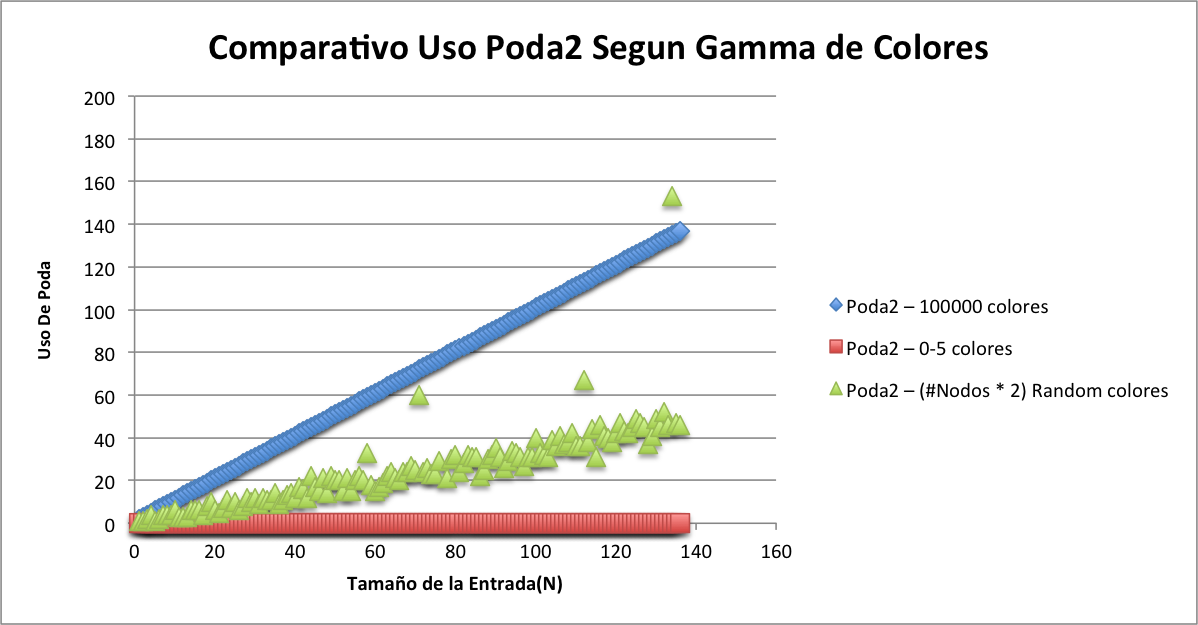
\includegraphics[width=140mm]{ejercicio2/ej2-comparativo-poda2-gammacolores.png}
\centering
\caption{Comparacion Uso de poda2 segun cantidad de colores posibles por nodo}
\label{overflow3}
\end{figure}\\

Este segundo grafico nos da la pauta de que sucede al reves que la anterior poda. Si los colores son muy dispersos, es probable que encontremos un color tal que ningun vecino mio lo contenga. Asimismo, si mi dispersion es muy baja, es altamente probable que los colores se repitan y no pueda descartar nada. En el medio tenemos la situacion donde tenemos una buena dispersion, sin embargo no es tan exagerada ni para un lado ni para el otro. De esa manera vemos que nuestro algoritmo utiliza mucho la poda2 siempre y cuando la variedad en la eleccion de los colores sea alta.\\|\\

\pagebreak
Ahora que sabemos que ambas podas son efectivas en cuanto a su uso, querriamos ver que sucede en cuanto al tiempo de ejecucion: si bien ambas se utilizan, es posible que ninguna o alguna de ellas no mejore visiblemente el tiempo de ejecucion.\\
En el siguiente grafo veremos los tiempos de ejecucion para un grafo cuyos colores no son dispersos

\begin{figure}[h!]
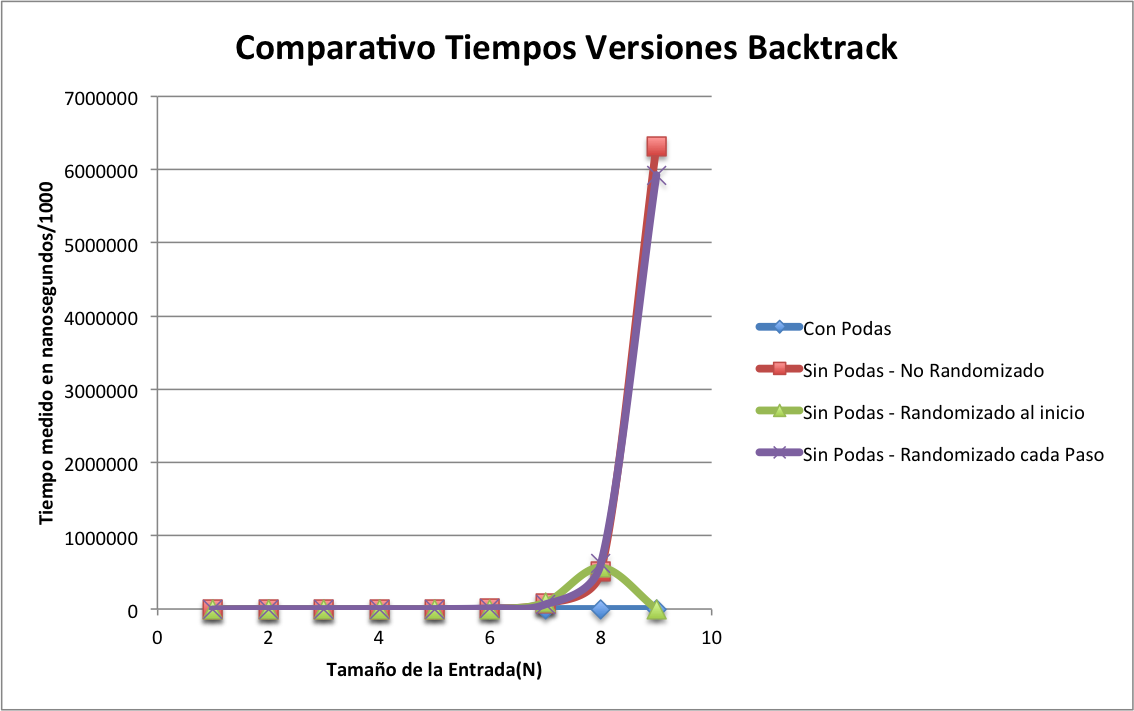
\includegraphics[width=140mm]{ejercicio2/ej2-comparativo-versionespng.png}
\centering
\caption{Comparacion Tiempos de ejecucion Poda vc No poda Colores no dispersos}
\label{overflow3}
\end{figure}
\\
\\

Lo que vemos es que si los colores estan poco distribuidos, el no utilizar la poda produce que los tiempos se vayan muy rapido hacia arriba. Siempre que utilicemos las podas el tiempo de ejecucion en comparacion a el tiempo versus sin podas es muchisimo menor. Asimismo vemos que justo el caso de color verde randomizo de una manera agradable y se acerco a la poda2 por ende su tiempo disminuyo considerablemente.\\

\pagebreak
Ahora veamos que sucede si tenemos los colores distribuidos:

\begin{figure}[h!]
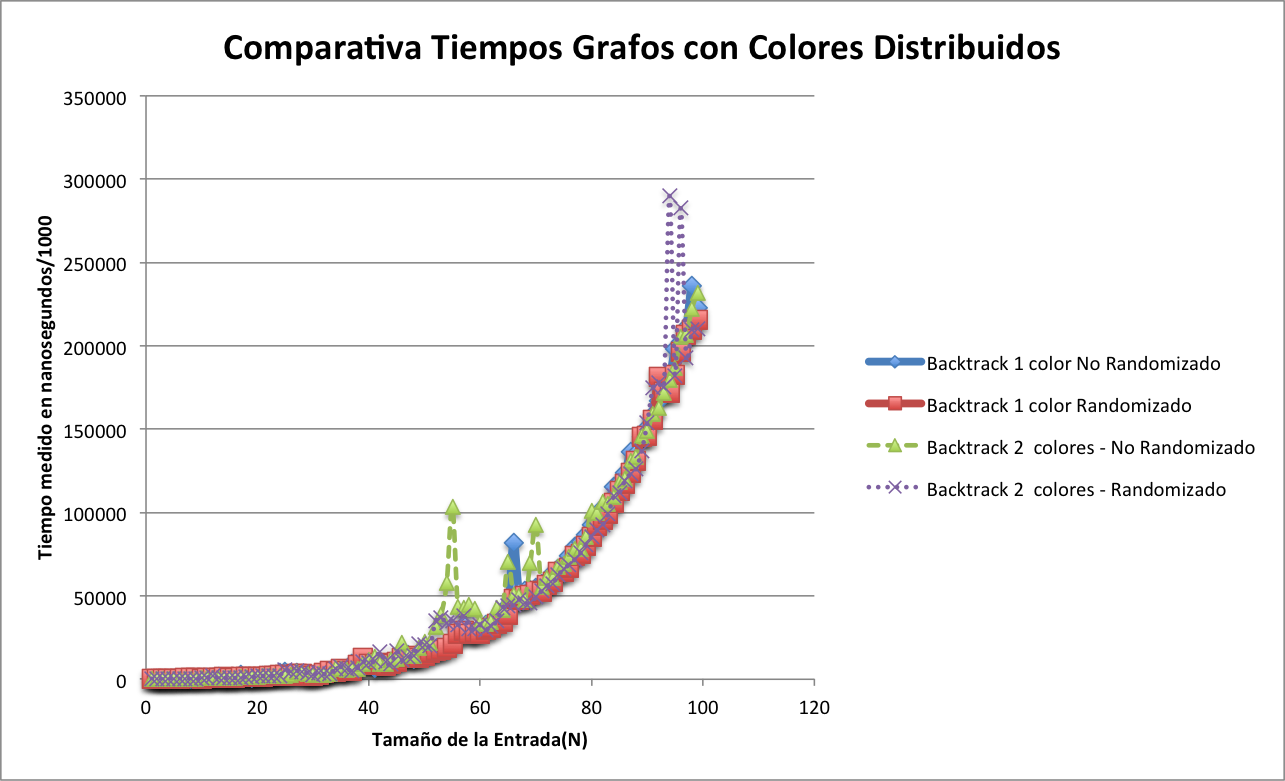
\includegraphics[width=140mm]{ejercicio2/ej2-comparativa-tiempos-colores-distribuidos.png}
\centering
\caption{Comparacion Uso de poda2 en relacion al tamanio de entrada(n+1 colores por nodo}
\label{overflow3}
\end{figure}

\\
\\
Lo que apreciamos es que si los colores estan distribuidos, entonces no importa que tipo de backtrack usemos. Si intentamos setear 2 colores para utilizar el ejercicio 1 o si o solo seeteamos 1 color para seguir con el backtrack, al tener los colores distribuidos, siempre entramos por la poda2, por lo que el tiempo de ejecucion se comparta mas o menos siempre de la misma manera. 
\pagebreak
\pagebreak
\section{Ejercicio 3}
\subsection{Problema}
Dise\~nar e implementar una \textbf{heur\'istica constructiva golosa} para List Coloring y desarrollar los siguientes puntos:\\

a) Explicar detalladamente el algoritmo implementado.\\

b) Calcular el orden de complejidad temporal de peor caso del algoritmo.\\

c) Describir instancias de List Coloring para las cuales la heur\'istica no proporciona una soluci\'on \'optima. Indicar qu\'e tan mala puede ser la soluci\'on obtenida respecto de la soluci\'on factible.\\

d) Realizar una experimentaci\'on que permita observar la performance del algoritmo en t\'erminos de tiempo de ejecuci\'on en funci\'on del tama\~no de entrada.\\
\subsection{Explicaci\'on y desarrollo del problema}


 A la hora de pensar una heruistica golosa, la mas simple y rapida podria ser pararse sobre un nodo al azar, elegir un color al azar y luego seguir con sus vecinos. Sin embargo esto podria generar muchisimos conflictos ya que depende estrictamente de la aleatoriedad con que elegimos los nodos y los colores. Lo que veremos a contiuacion, es que a esta herusitica recien mencionada se le pueden hacer pequenias mejoras tal que mejoren la performance del resultado.\\
 Empezaremos de un nodo al azar y recorreremos sus colores. Para cada uno de ellos iteraremos los vecinos del nodo en cuestion y preguntaremos si este vecino ya esta pintado y su color es el mismo en el cual estamos iterando. En este caso el color es invalido. En caso de que no este pintado, nos preguntaremos, si tiene mas de 1 color disponible y nuestro color en cuestion pertenece a la lista de colores de ese vecino, entonces tambien es invalido. En cualquier otro caso sera valido. Los casos donde puede ser valido es si el color en cuestion no se encuentra entre los colores disponibles del vecino en donde estamos iterando.\\ Ademas, puede suceder en un grafo poco feliz que nuestro nodo N tenga los colores 1,2,3 y que tenga 3 vecinos A,B,C cuyos unicos colores sean 1,2,3 respectivamente. En este caso decidimos que al salir del ciclo (es decir el ciclo no pudo decidir ningun color), pintamos al nodo N con el ultimo color de la lista. En este caso, por descarte, tambien sera un color valido.\\
 Luego de pintar el nodo, seguiremos iterando por los demas nodos.\\\\
 
 
 Esta heuristica tiene un defecto muy importante y puede comportarse muy mal en determinados casos.\\
 Imaginemos un grafo donde exista un coloreo valido, sin embargo para cada nodo, su color valido este en el final de la lista. Es posible que, par algun nodo, exista un color de la lista que sea valido localmente, sin embargo a gran escala no seria el correcto. Nuestro algoritmo recorre la lista de colores en orden, de manera tal que primero se encontraria con el color incorrecto, lo seteearia y el coloreo quedaria equivocado.
 
 La segunda heuristica pasa por exactamente el mismo proceso, salvo que a la hora de iterar los colores, no se queda con el primer color que es valido, sino que al encontrar un color valido, chequea que sucederia con sus vecinos si pintamos el nodo de ese color. Mas precisamente, para cada color A, cuenta la cantidad de colores que le que quedan disponible a cada vecino sin contar a A y los suma en una variable "posibilidades". Luego, elegira el color tal que si yo lo elijo, tengo la mayor cantidad de posibilidades para elegir entre mis vecinos. Esta heuristica, a priori, tiene mas posibilidades de encnontrar el optimo dentro de una vecindad en particular ya que antes de setear un color, revisa si es el que maximiza las posibilidades. Sin embargo, esta heurisitica podria funcionar muy mal a la hora de ver mas a largo plazo.\\\\
 Lo que podemos apreciar en el ejemplo es que esta heuristica puede funcionar tan mal como nosotros querramos.
\begin{center}

\usetikzlibrary{positioning}
\tikzset{main node/.style={circle,fill=blue!20,draw,minimum size=1cm,inner sep=0pt},
            }

  \begin{tikzpicture}
    \node[main node] (1) {$V/R$};
    \node[main node] (2) [below left = 1.5cm and 1.2cm of 1]  {$A/V$};
    \node[main node] (3) [below right = 1.5cm and 0.0cm of 1] {$A/R$};
    \node[main node] (4) [below right = 2.3cm and 0 cm of 3] {$R$};
    \node[main node] (5) [below right = 1cm and 0.7cm of 3] {$R$};
    \node[main node] (6) [right = 0.7cm  of 3] {$R$};

    \path[draw,thick]
    (1) edge node {} (2)
    (2) edge node {} (3)
    (3) edge node {} (4)
    (6) edge node {} (3)
    (5) edge node {} (3);
    %%
    
\end{tikzpicture}

\caption{NodosEstado de A y B.}
\end{center}

 si bien el grafo tiene un coloreo optimo donde 0=v 1=r 2=a 3...=r, El proceso por el que pasa nuestro algoritmo es el siguiente:
 \begin{enumerate}
 \item Si elijo verde cuantas posibilidades tengo? Los vecinos de 0 son 1 y 2 por ende: Posibilidades = #(colores(1)-verde)+#(colores(2)-verde) = 1+1=2
 \item Si elijo azul cuantas posibilidades tengo? Los vecinos de 0 son 1 y 2 por ende: Posibilidades = #(colores(1)-azul)+#(colores(2)-azul) = 1+2=3
 \item Elijo azul y avanzo hacia el nodo 1.
 \item El nodo 1 ahora solo tiene un color disponible que es el rojo, por ende lo seteo de tal manera y voy a sus vecinos.
 \item Todos los vecinos de 1 son unicamente de color rojo, por ende por cada vecino que tenga tal que solo puede ser pintado de rojo, el algoritmo encontrara un conflicto.
 \end{enumerate}\\

 
Nuestra hipotesis a analizar en los tests, es que para grafos generados pseudo-aleatoriamente y con una variedad amplia de colores, la segunda heuristica tiene mayor tiempo de ejecucion respecto de la primera ya que debe recorrer todos los colores del nodo para encontrar el que maximiza las posibilidades, pero encontrara un resultado mas cercano la optimo. Mientras menos dispersos esten los colores, mas cercanos creemos que seran los tiempos de ejcucion. \\

Una vez analizada la hipotesis, se nos ocurrio dessarrollar una tercer heuristica que es simplemente una variante de la recien mencionada:
Decidimos entonces desarrollar una heurisita que funcione igual que la segunda pero que recorra un determinado X$\div$ de los colores, siempre y cuando al llegar al X$\div$ haya encontrado un color valido. En caso de no encontrarlo, seguira iterando los colores hasta hacerlo. No sabemos que comportamiento tendra, pero nuestra hipotesis es que se situara en el medio de las otras dos, es decir que sera mejor que la primera y peor que la segunda a la hora de analizar la cantidad de conflictos pero a medida que ese porcentaje aumente, el tiempo de ejecucion aumentara tambien.

\subsection{Pseudo-C\'odigo}

\begin{verbatim}
solve()
FOREACH materias(grafo) as materia   // O(cantidad(Materias))
    IF cantidadColores(materia) == 1 THEN  // 
        colorFinal(materia) = color(materia);  // O(1)
    ELSE
    var Boolean seteeColor = false;            // O(1)
    int i; int color = 0;                     // O(1)
        FOR i desde 0 hasta cantidadColores(materia) Y !seteeColor   // O(cantidadColores(materia)
            boolean colorValido = true;
            color =  color(materia,i);
            FOREACH  vecinos(materia) as vecino                      // O(#vecinos(materia))
                IF noTieneColorFinal(vecino) THEN
                    IF (colores(vecino) != 1 && esta(color,colores(vecinos))){ // O(cantidadColores(materia)
                        colorValido = false;
                    ENDIF
                ELSE

                IF colorFinal(vecino) == color
                    colorValido = false;
                ENDIF

                IF colorValido 
                    seteeColor = true;
                    setearColorFinal(materia, color)
                ENDIF
            ENDFORECH
        ENDFOR
    IF ! seteeColor
        setearColorFinal(materia, color)   // O(1)
    ENDFOR
ENDFOREACH
\end{verbatim}

\subsection{Justificaci\'on y Complejidad}
\\
Como pudimos ver en la seccion anterior, podemos dar una analisis de complejidad en un peor caso, tomando cotas superiores en varios puntos del algoritmo.\\
Lo que podemos decir que es que para cada materia, haremos muchas operaciones de orden constante y un FOR que recorre todos los colores de la materia. Dentro de ese ciclo, volvemos a usar operaciones del orden constante y utilizamos otro clcio que involuchra todos los vecinos de la materia en cuestion.\\

Simplificando la complejidad del algoritmo, se observa que es un "Para todos las materias => Para Todos los colores de la materia => Para todos los vecinos de la materia => Operaciones O(1)" \\. La cantidad de colores de la materia esta acotado por la maxima cantidad de colores que tenga una materia, que por simplicidad llamaremos M. La cantidad de vecinos esta acotada tambien por la cantidad de materias en todo el grafo (ninguna materia puede tener mas vecinos que todas las materias del grafo), Por ende la complejidad viene dada por O(Cantmaterias*M*CantMaterias)\subset O(Cantmaterias^2 * M)


\subsection{Tests y Performance}

En esta seccion vamos a realizar distintas pruebas:
\begin{enumerate}
 \item Para un grafo que sepamos que funciona mal en la H1, veremos su funcionamiento en H2 en relacion a la cantidad de conflictos.
 \item Para un grafo que sepamos que funciona mal en la H2, veremos su funcionamiento en H1 en relacion a la cantidad de conflictos.
 \item Analizaremos como se comporta un grafo aleatorio en relacion a los conflictos para H1 y H2 y los tiempos de ejecucion.
 \item Una vez comparadas las heuristicas H1 y H2, veremos como funciona el tema conflcitos y los tiempos de ejecucion en la H3 con distitntas variantes:
 \begin{enumerate}
 \end{enumerate}\\
 
Por otro lado veremos como crece la complejidad y la cantidad de conflicos del problema al aumentar la cantidad de aristas para cada una de nuestras heuristicas. \\
\begin{figure}[h!]
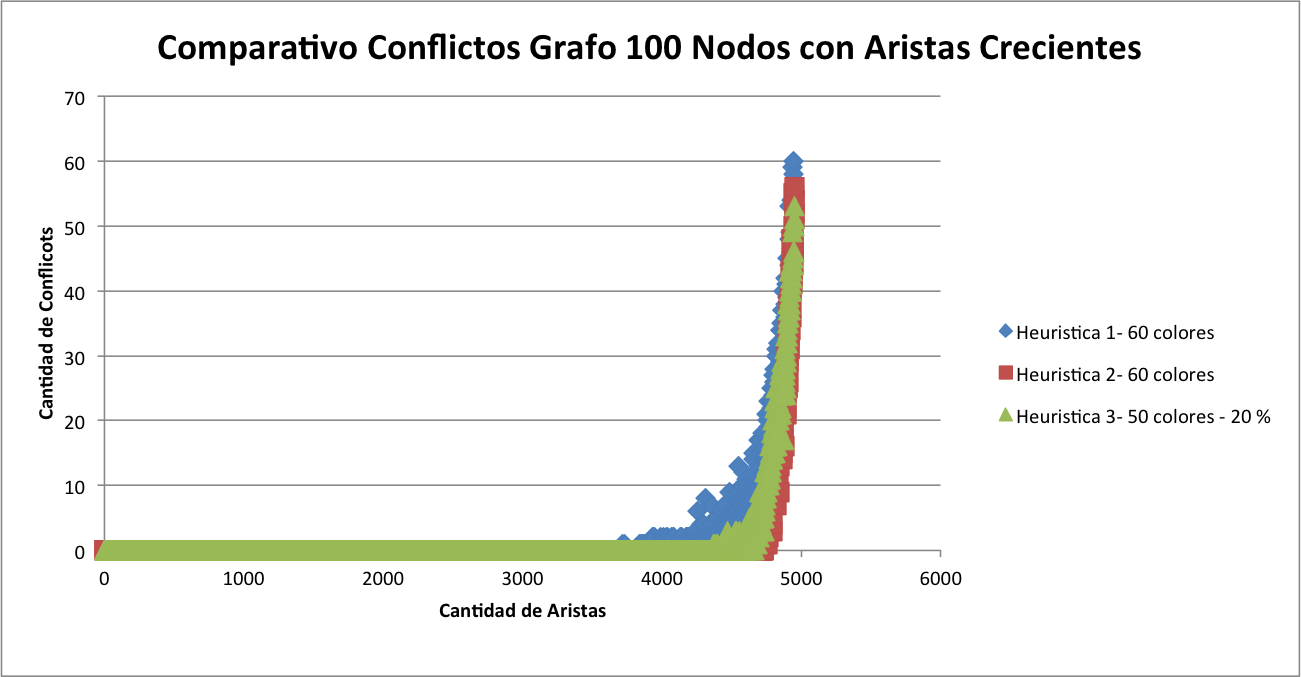
\includegraphics[width=140mm]{ejercicio3/ej3-comparativo-grafo100-conflicto.png}
\centering
\caption{comparativa conflictos aumento de aristas}
\label{overflow3}
\end{figure}
 \pagebreak
\\ 
\begin{figure}[h!]
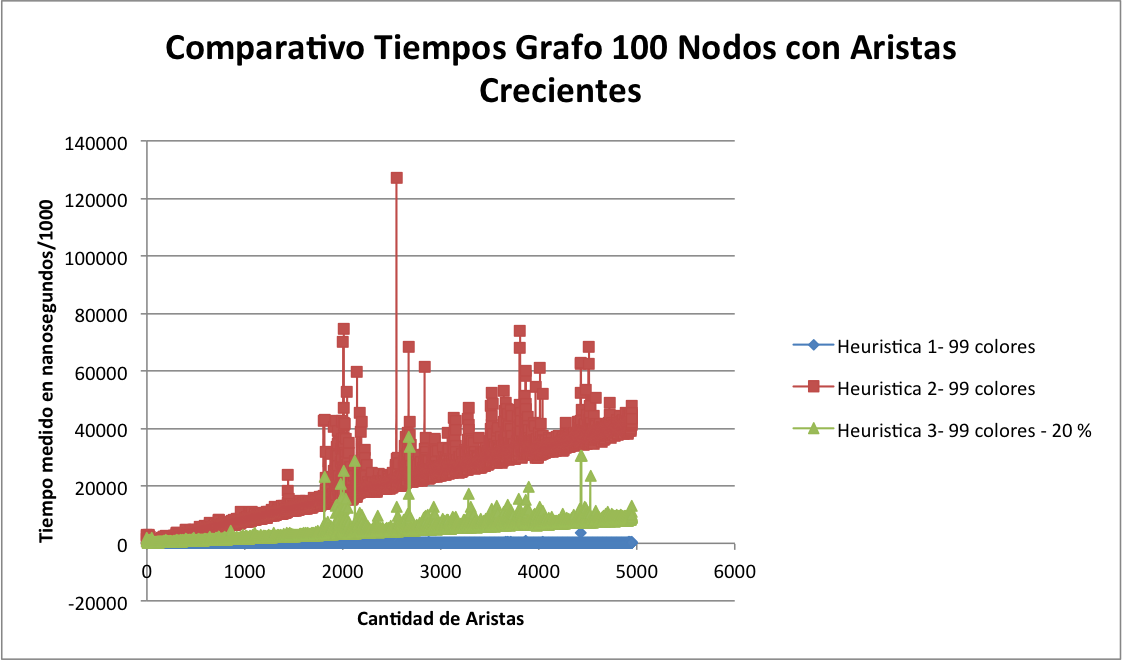
\includegraphics[width=140mm]{ejercicio3/ej3-comparativo-grafo100-tiempo-99colores.png}
\centering
\caption{comparativa tiempos aumento de aristas 100 colores}
\label{overflow3}
\end{figure}
\\

\begin{figure}[h!]
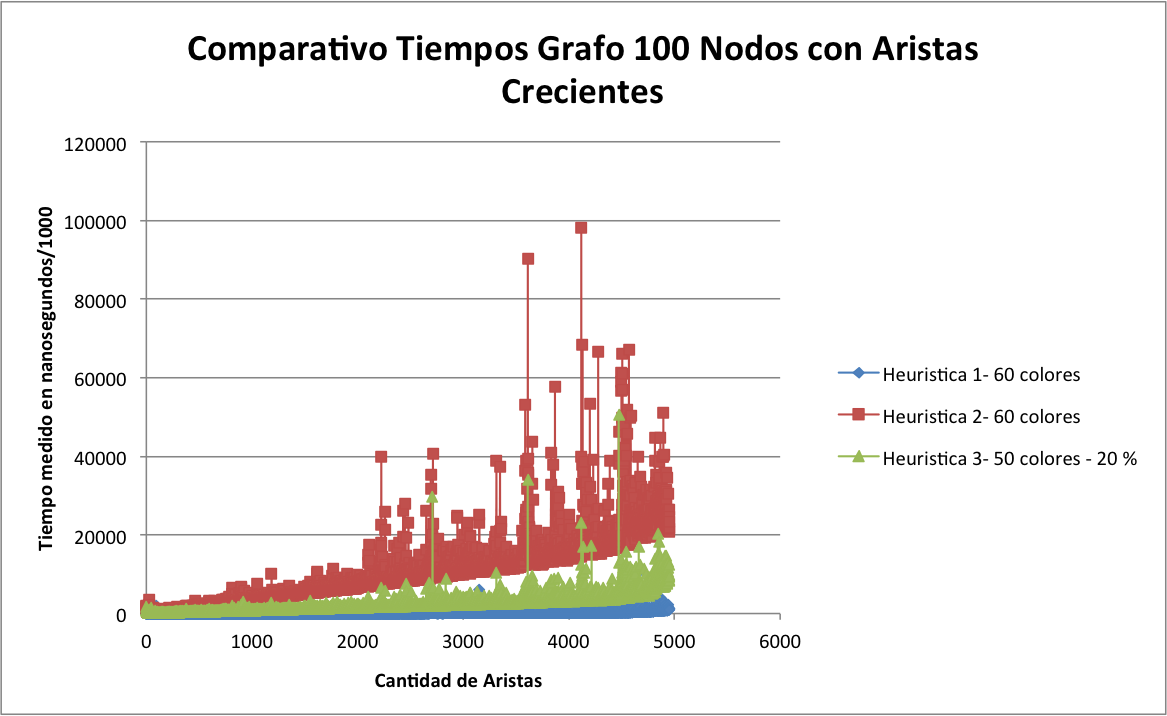
\includegraphics[width=140mm]{ejercicio3/ej3-comparativo-grafo100-tiempo.png}
\centering
\caption{comparativa tiempo aumento de aristas 50 colores}
\label{overflow3}
\end{figure}
\\
\pagebreak
\newpage
\begin{figure}[h!]
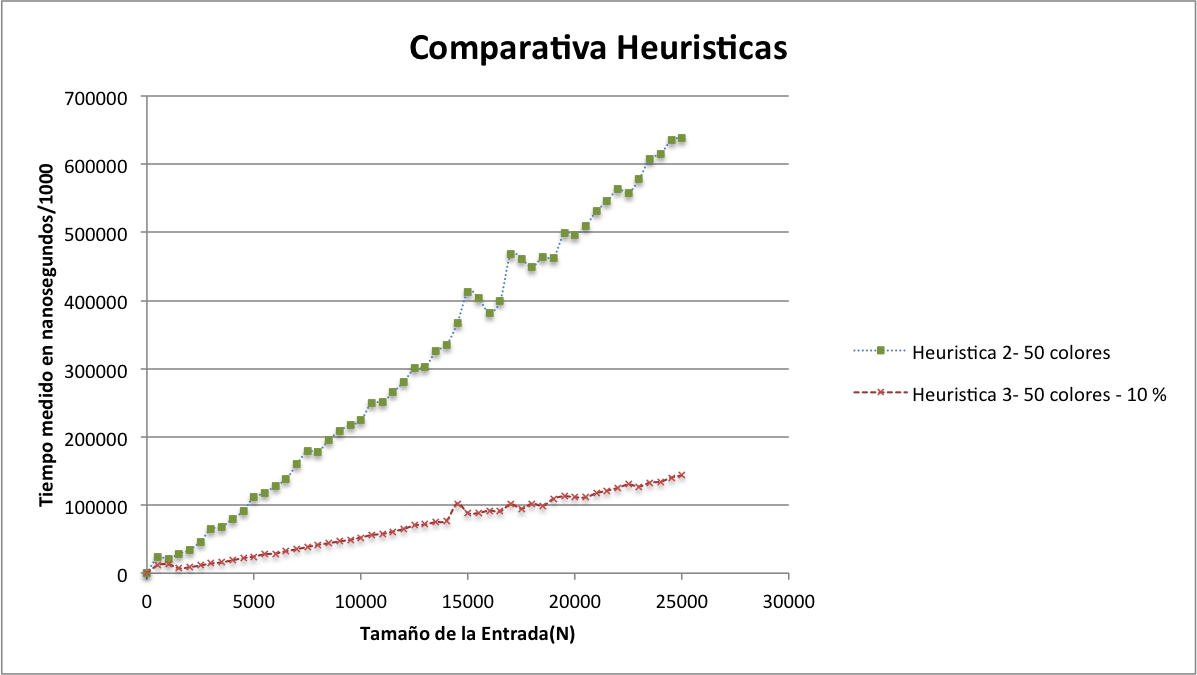
\includegraphics[width=140mm]{ejercicio3/ej3-comparativo-10.png}
\centering
\caption{Comparacion tiempo h2 Vs tiempo h3 10}
\label{overflow3}
\end{figure}



Lo que podemos apreciar es que la complejidad del algoritmo depende primordialmente de la cantidad de aristas ya que esta modifica la cantidad de vecinos de cada nodo. Esto sucede por que en el algoritmo vemos que la mayoria de cuentas se producen dentro del ciclo que reocrre los vecinos. Para un nodo que no tiene vecinos, simplente seteamos un color, mientras que por cada vecino tendremos que chequear varias cosas que si bien son O(1), suman.\\
Ahora analizaremos lo antes mencionado. \\
1 y 2)\\ Mediante la siguiente tabla podemos ver que encontramos una familia de grafos y de distribuciones de colores tal que si bien tienen coloreos validos, nuestras heuristicas los rompen tanto como quieran.\\
\begin{tabular}{| l | c | r |}
  \hline
Grafo Solucion Optima Al Final  & GrafoRompe Heuristica 2 & Aleatorio 100 nodos \\ \hline
6  & 0 & 169\\ \hline
1  & 10 & 92\\ \hline
\end{tabular}

\\Para la primer heuristica, si para cada nodo, el color que corresponde al coloreo valido se encuentra en el ultimo lugar, primero revisara todos los anteriorir y en caso de encontrar uno que localmente sirva, no llegara a revisar el color optimo y lo perdera.\\
Por otro lado, como mencionamos en la explicacion, la heuristica dos puede funcionar infinitamente mal (ver ejemplo).\\
Ademas vemos que para un grafo aleatorio de 100 nodos y relativamente denso, la heuristica dos es un poco mas eficiente que la uno en cuanto a cantidad de conflictos.

3) Veamos que si todos los nodos tienen un solo color, las heuristicas tardaran lo mismo ya que la segunda heuristica no debe recorrer todos los colores del nodo (tiene uno solo).\\

\begin{figure}[h!]
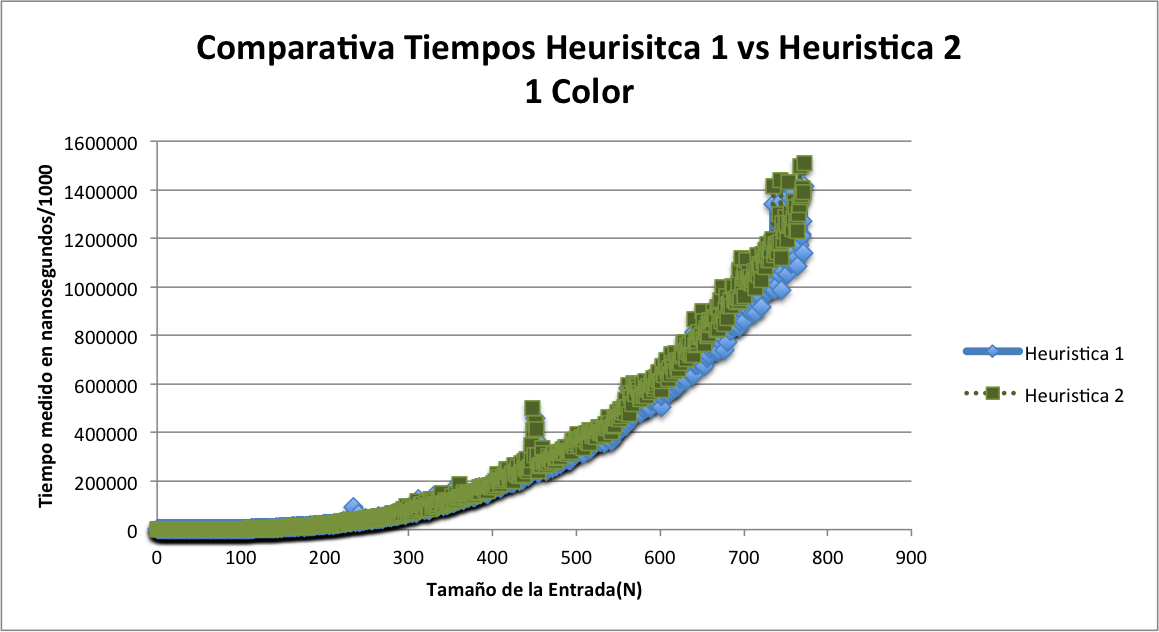
\includegraphics[width=140mm]{ejercicio3/ej3-comparativo-eu1-eu2-grafoCreciente-tiempo-1color.png}
\centering
\caption{Comparacion tiempo h1 Vs tiempo h2 1 color por nodo}
\label{overflow3}
\end{figure}


Ahora veamos que sucede si le ponemos N colores:\\

\pagebreak
\begin{figure}[h!]
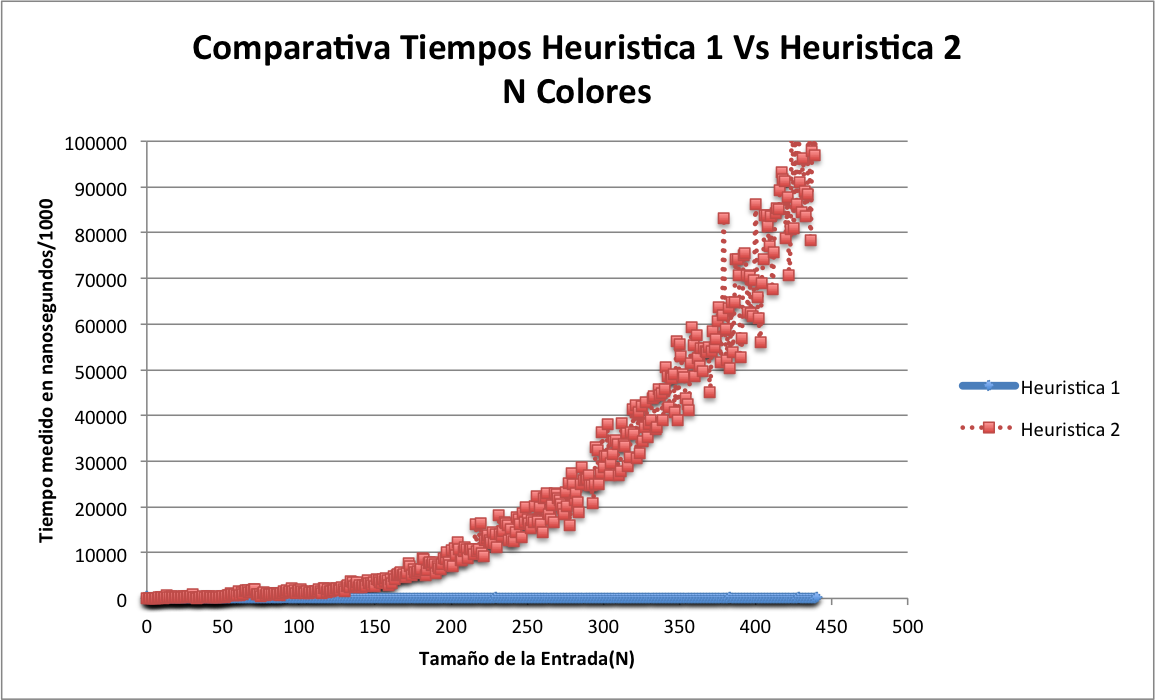
\includegraphics[width=140mm]{ejercicio3/ej3-comparativo-eu1-eu2-grafoCreciente-tiempo.png}
\centering
\caption{Comparacion tiempo h1 Vs tiempo h2 N colores por nodo}
\label{overflow3}
\end{figure}

La conclusion que sacamos es que al tener muchos colores, la H1 encontrara un color valido en algun momento y no llegara a revisar toda la lista de colores por completo como si lo hace la H2. Con respecto a los conflictos, el analisis esta plasmado en el cuadro de 1 y 2.\\
4) Antes de empezar decidimos no utilizar la H3 10porciento para los grafos con 10 colores ya que carece de sentido. Tambien aclararemos que el grafo utilizado es un grafo de 25k nodos no tan denso.\\


\begin{figure}[h!]
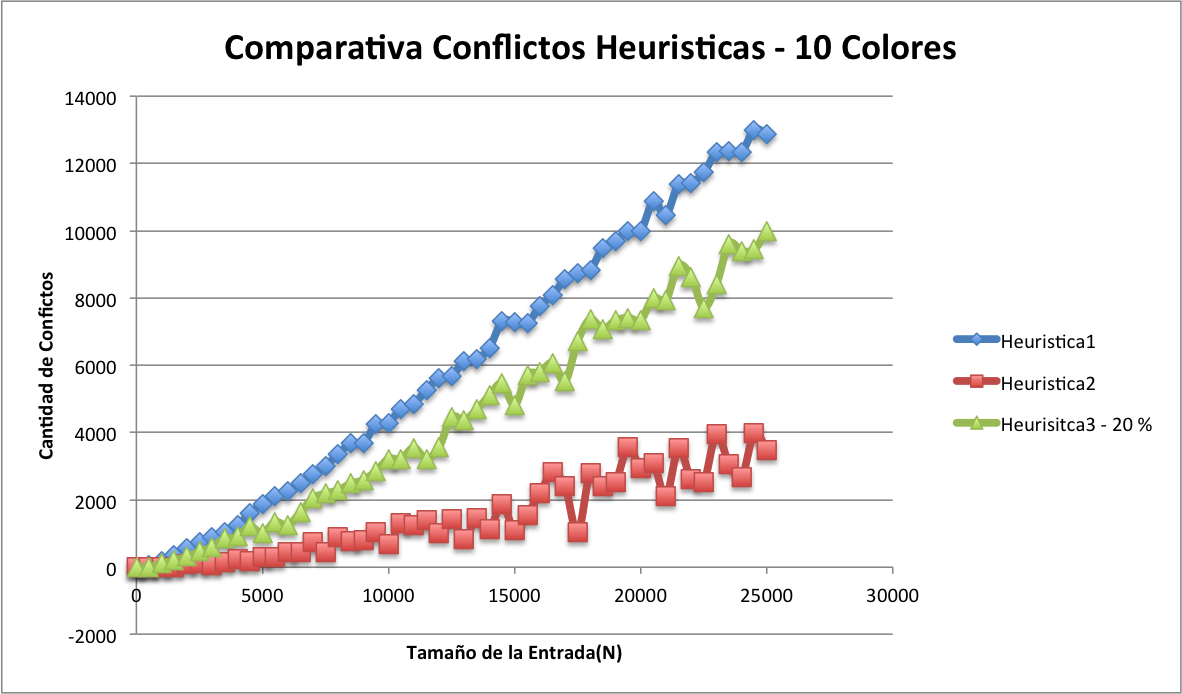
\includegraphics[width=140mm]{ejercicio3/ej4-comparativa-conflictos-10.png}
\centering
\caption{Comparacion conflictos h1 vs h2 Vs h3 10 colores por nodo}
\label{overflow3}
\end{figure}

\pagebreak

\begin{figure}[h!]
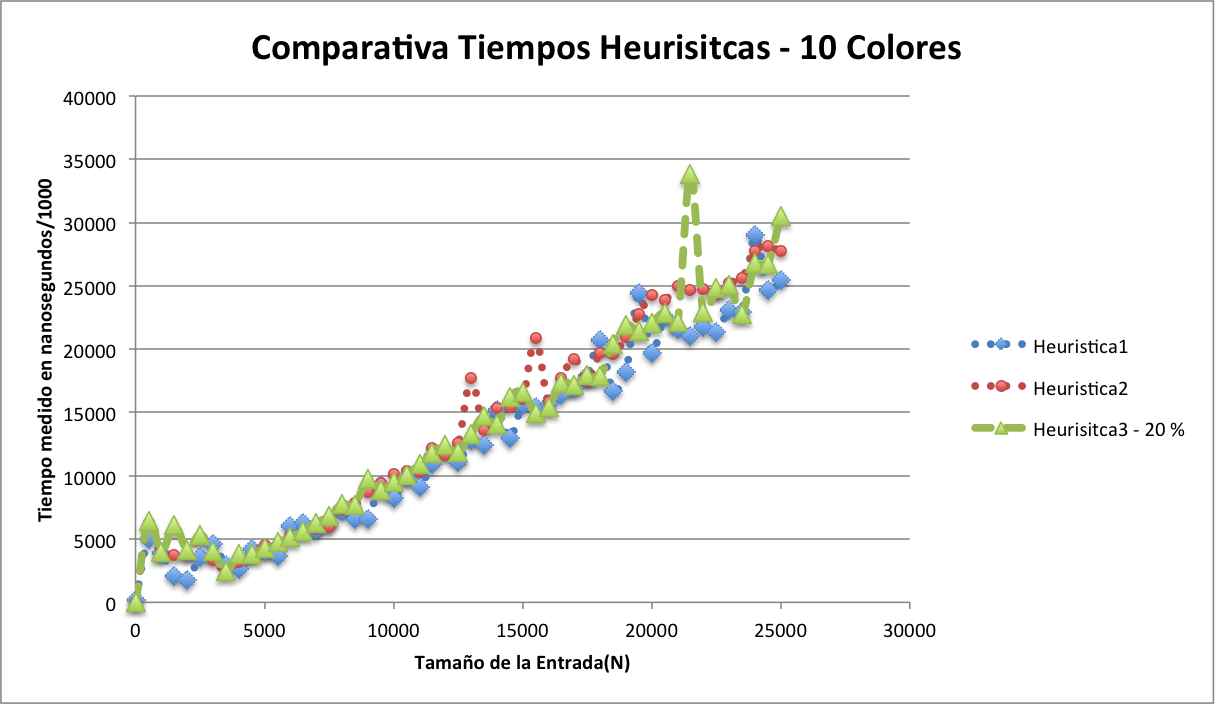
\includegraphics[width=140mm]{ejercicio3/ej4-comparativa-tiempos-10.png}
\centering
\caption{Comparacion tiempos h1 vs h2 Vs h3 10 colores por nodo}
\label{overflow3}
\end{figure}
\\
\\
Lo que podemos apreciar en los anteriores graficos es que cuando tenemos pocos colores, el tiempo de ejecucion es similiar para las tres heuristicas. Como estamos en un grafo de muchos nodos, es muy probable que con 10 colores, siempre encuentres un conflicto, por lo que la H1, tendera a revisar muchos colores. La H2, revisa todos los colores siempre y por otro lado la h3 solo revisa un porcentaje pero ya que sucede lo mismo que con la H1, tiende a revisar la mayoria de los colores. En relacion a los conflictos, vemos que la H2 es la que mejor se comporta ya que siempre que localmente haya un color valido, lo seteara mientras que la H1 se quedara con el primero que encuentre que sea valido.\\
\\
\\
\begin{figure}[h!]
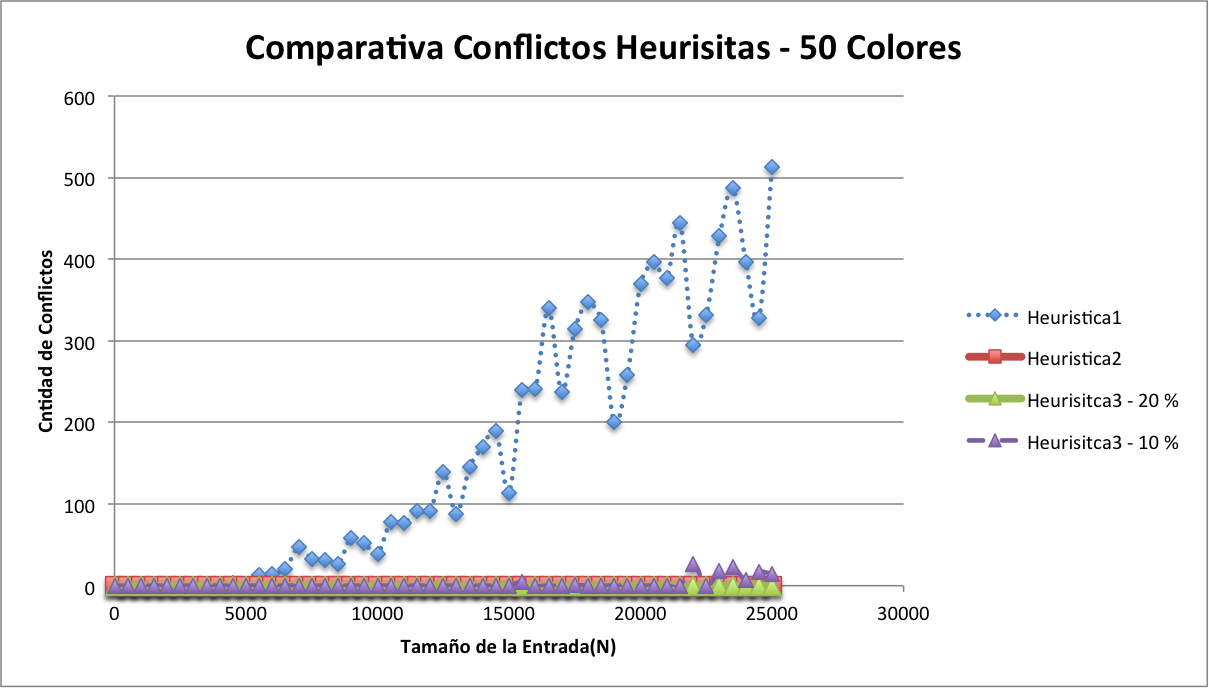
\includegraphics[width=140mm]{ejercicio3/ej4-comparativa-conflictos-50.png}
\centering
\caption{Comparacion conflictos h1 vs h2 Vs h3 50 colores por nodo}
\label{overflow3}
\end{figure}
\\
\\
\begin{figure}[h!]
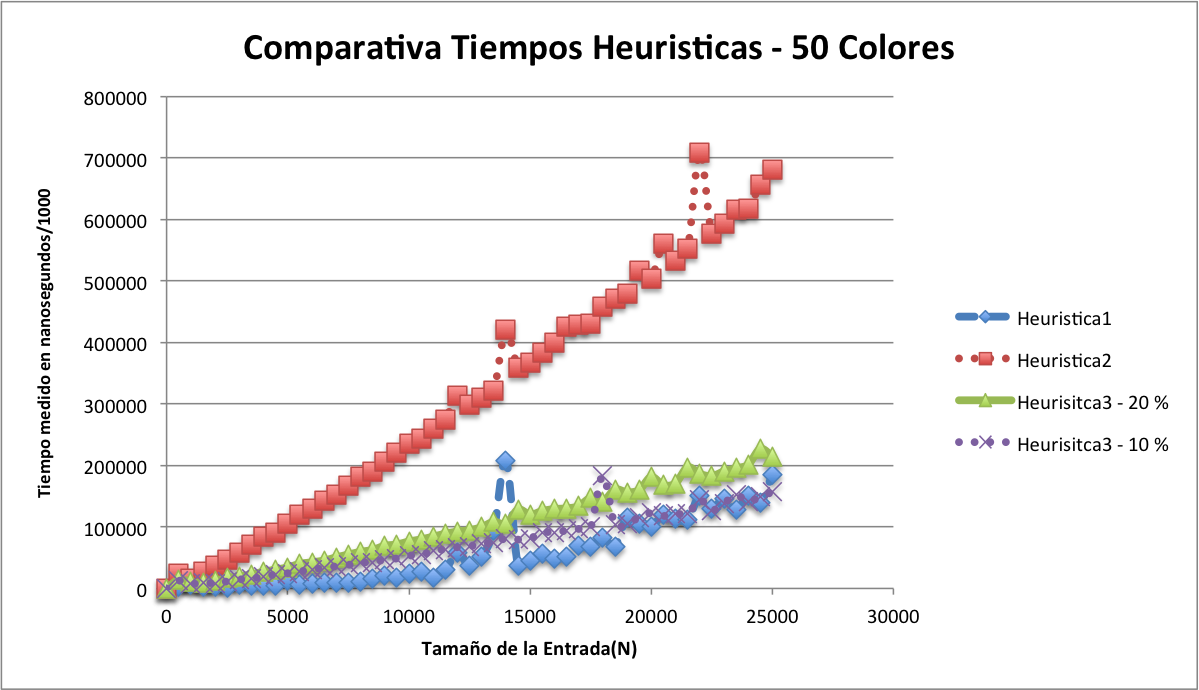
\includegraphics[width=140mm]{ejercicio3/ej4-comparativa-tiempos-50.png}
\centering
\caption{Comparacion tiempos h1 vs h2 Vs h3 50 colores por nodo}
\label{overflow3}
\end{figure}

\pagebreak
Si tenemos muchos colores ( Hicimos el analisis para 50 colores y 0,5$\%$ de densidad) la H2 debera recorrerlos todos y eso hara demasiada diferencia ante la H1 donde recorrera unicamente hasta encontrar un color valido. Paliativamente tenemos la H3 que como muy bien indica el grafico, mientras mas alto sea el porcentaje de colores a revisar, mas tiempo tardara en hallar la solucion.\\
A la hora de analizar el tema de los conflictos, al igual que antes la H1 no funiona muy bien ya que nos encuentra muchisimos conflictos. Sin embargo vemos como las demas heuristicas si bien han pagado un tiempo de ejecucion mayor, nos encontraron coloreos validos.
\pagebreak
\pagebreak
\section{Ejercicio 4}
\subsection{Problema}
Dise\~nar e implementar una \textbf{heur\'istica de b\'usqueda local} para List Coloring y desarrollar los siguientes puntos:\\

a) Explicar detalladamente el algoritmo implementado. Plantear al menos dos vecindades distintas para la b\'usqueda.\\

b) Calcular el orden de complejidad temporal de peor caso de una iteraci\'on del algoritmo de b\'usqueda local (para las vecindades planteadas). Si es posible, dar una cota superior para la cantidad de iteraciones de la heur\'istica.\\

c) Realizar una experimentaci\'on que permita observar la performance del algoritmo comparando los tiempos de ejecuci\'on y la calidad de las soluciones obtenidas, en funci\'on de las vecindades utilizadas y elegir, si es posible, la configuraci\'on que mejores resultados provea para el grupo de instancias utilizado.\\

\subsection{Explicaci\'on del problema}
Para comenzar, decidimos utilizar una de las heurisitca del ejercicio3 de manera tal de conmenzar en una subsolucion mas cercana al optimo que una solucion aleatoria. Luego de eso nos preguntaremos si ya esta resuelto, devolvemos ese grafo, sino, llamaremos a nuestra funcion que resuelve. Definiremos el vecindario de cada subsolucion como los distintos grafos tal que cada subsolucion intenta arreglar un conflicto determinado. Por ejemplo si tenemos una subsolucion con 8 conflictos, tendremos 8 vecinos de manera tal que cada vecino$_{i}$ representa al grafo que intenta arreglar el conflicto i. Luego veremos si el minimo(CantConflictos(vecino$_{i}$)) es mayor, menor o igual a la cantidad de conflictos de nuestra subsolucion. Si el mejor de mis vecinos es mayor, significa que por esa rama no puedo mejorar y por ende cortamos la ejecucion quedando como solucion nuestra subsolucion. Si es igual cambiaremos la subsolucion y seguiremos adelante. Sin embargo si sucede que durante 5 iteraciones seguidas nuestro algoritmo no consiguio mejorar, decidimos que esa es nuestra mejor solucion. En caso de que sea menor, haremos un cambio de subsolucion y setearemos la cuenta de repeticiones a 0.\\
Ahora veremos como hacemos conseguir solucionar un conflicto para una determinada subsolucion. Dada una solucion A que tiene conflictos entre los nodos B y C, Miro todos los vecinos de B y me quedo con el conjunto de colores con los que estan pintados. Luego miraremos si existe algun color en B tal que no pertenezca a ese conjunto y en caso de ser cierto, pintaremos a B de ese color. En caso de ser falso, significa que no tengo ningun color en B tal que si lo pinto de ese color, no me produzca ningun conflicto. Si luego de este proceso no pudimos resolver el conflicto, lo intentaremos de la misma manera pero para el nodo C. Luego, si ninguno pudo, mantendremos la misma cantidad de conflictos.\\
Aca veremos un caso donde la busqueda local nos solucionara un conflicto.\\
Posible Caso en el que la busqueda local soluciona un conflicto:


\usetikzlibrary{positioning}
\tikzset{main node/.style={circle,fill=blue!20,draw,minimum size=1cm,inner sep=0pt},
            }

  \begin{tikzpicture}
    \node[main node] (1) {$V/R$};
    \node[main node] (2) [below left = 1.5cm and 1.5cm of 1]  {$V/R/A$};
    \node[main node] (3) [below right = 1.5cm and 1.5cm of 1] {$V/R$};
    

    \path[draw,thick]
    (1) edge node {} (2)
    (2) edge node {} (3)
    (3) edge node {} (1);
    
\end{tikzpicture}

Si la heuristica1 por ejemplo hace el analisis empezando por el nodo de abajo a la izquierda que tiene 3 colores y elige el color Verde o Rojo, vamos a suponer el verde, luego continua con el que esta a su derecha, el algoritmo determina que se debe elegir el color rojo ya que sino habria conflictos. Luego al analizar el nodo superior descubre que no es posible elegir un color ya que los dos generan un conflicto, para efectos de este ejemplo vamos a suponer que elige el verde. El grafo que nos queda es el siguiente:

\tikzset{main node/.style={circle,fill=blue!20,draw,minimum size=1cm,inner sep=0pt},
            }

  \begin{tikzpicture}
    \node[main node] (1) {$V$};
    \node[main node] (2) [below left = 1.5cm and 1.5cm of 1]  {$V$};
    \node[main node] (3) [below right = 1.5cm and 1.5cm of 1] {$R$};
    

    \path[draw,thick]
    (1) edge node {} (2)
    (2) edge node {} (3)
    (3) edge node {} (1);
    
\end{tikzpicture}

Este grafo tiene un conflito que es resoluble con la busqueda local, ya que al analizar el primer nodo es posible elegir un nuevo color, el Amarillo, lo cual al cambiarlo nos mejoraria nuestro coloreo quedando el siguiente coloreo optimo.

  \begin{tikzpicture}
    \node[main node] (1) {$V$};
    \node[main node] (2) [below left = 1.5cm and 1.5cm of 1]  {$A$};
    \node[main node] (3) [below right = 1.5cm and 1.5cm of 1] {$R$};
    

    \path[draw,thick]
    (1) edge node {} (2)
    (2) edge node {} (3)
    (3) edge node {} (1);
    
\end{tikzpicture}\\
\\
Como segundo vecindario tomamos los mismos conflictos que en el primero pero a diferencia del anterior no se trabaja individualmente sobre un solo nodo, sino que se trabaja sobre todos los nodos conflicto que, habiendo cambiado por un color libre, mejoraron la solucion anterior, sobre esto se entrara mas en detalle en la experimentacion(ver secci\'on 4.6).
\subsection{Desarrollo del problema}

\subsection{Pseudo-C\'odigo}

\begin{verbatim}
public Coloreo solve() {
        Listacolores = listaColores()
        ej3.solve() // Se puede elegir cualquier solucion de alguna de las heuristicas
        int [] vectorColores = ej3.getColoreo() //O(Ej3) Con alguna de las heuristicas

        FOR i desde 0 hasta vectorColores.length DO //O(CantColores)
            Color actual = Nuevo Color(vectorColores[i], i) //O(1)
            colores.add(actual); // O(1)
        ENDFOR

        coloreoActual = new Coloreo(grafo, colores) //O(%!!!!%

        IF coloreoActual.esValido() THEN //O(1)
            DEVOLVER coloreoActual
        ELSE
            DEVOLVER resolve(coloreoActual)
        ENDIF
}

private Coloreo resolve(Coloreo colores) {
    int noCambio = 0 //O(1)
    int cantidadSinMejorar = 5 //O(1)
    Coloreo nuevoColoreo //O(1)
    Coloreo mejorColoreo = colores //O(1)

    WHILE !mejorColoreo.esValido() && noCambio < cantidadSinMejorar //O(cotaBruta)
        nuevoColoreo = getProximoColoreo(mejorColoreo) //O(getProximoColoreo)

        IF nuevoColoreo.cantidadDeConflictos() <= mejorColoreo.cantidadDeConflictos() THEN //O(1)
            mejorColoreo = nuevoColoreo; //O(1)

            IF nuevoColoreo.cantidadDeConflictos() == mejorColoreo.cantidadDeConflictos() //O(1) THEN
                noCambio++ //O(1)
            ELSE
                noCambio = 0 //O(1)
            ENDIF
        ELSE
            noCambio = cantidadSinMejorar //O(1)
        ENDIF
    ENDWHILE
    DEVOLVER mejorColoreo
}


CotaBruta: Lo peor que puede suceder es que tengamos un grafo de N nodos tal que este 
pintado del mismo color y tenga N conflictos. Si cada
iteracion, intentamos solucionar 1 conflicto y lo logramos,
podriamos tener N iteraciones hasta llegar a un coloreo valido.\\
\\

Coloreo getProximoColoreo(Coloreo colores)
    Coloreo nuevoColoreo //O(1)
    Coloreo mejorColoreo = colores //O(1)

    FOREACH colores.getConflictos() AS c //O(CantidadConflictos) $\subset$ O(N)
        ArrayList<Color> nuevosColores = new ArrayList<Color>(colores.getColores()); //O(1)
        TreeSet<Integer> coloresOcupados = new TreeSet<Integer>(); //O(1)
        NodoMateria nodoActual = grafo.getMateria(c.getId()); //O(1)


        FOREACH nodoActual.getAdyacentes() AS vecino //O(CantVecinos) $\subset$ O(N)
            List<Color> coloresSeteados = colores.getColores(); //O(1)
            int color = coloresSeteados.get( vecino.getId() ).getColor(); //O(1)
            coloresOcupados.add(color); //O(1)
        ENDFOREACH

        ArrayList<Integer> coloresPosibles = Copia(nodoActual.getColoresPosibles())
        coloresPosibles.removeAll(coloresOcupados)

        IF ! coloresPosibles.isEmpty()
            Color actual = new Color(nodoActual.getId(), coloresPosibles.get(0));
            nuevosColores.set(nodoActual.getId(), actual);
            nuevoColoreo = new Coloreo(grafo, nuevosColores);
            IF nuevoColoreo.cantidadDeConflictos() <= mejorColoreo.cantidadDeConflictos()
                mejorColoreo = nuevoColoreo;
            ENDIF
        ENDIF
    ENDFOREACH

    DEVOLVER mejorColoreo
}

Como nueva vencindad se probo lo siguiente:

public Coloreo solveVecindad2() {
    Listacolores = listaColores()
    ej3.solve() // Se puede elegir cualquier solucion de alguna de las heuristicas
    int [] vectorColores = ej3.getColoreo() //O(Ej3) Con alguna de las heuristicas

    FOR i desde 0 hasta vectorColores.length DO //O(CantColores)
        Color actual = Nuevo Color(vectorColores[i], i) //O(1)
        colores.add(actual); // O(1)
    ENDFOR

    coloreoActual = new Coloreo(grafo, colores) //O(%!!!!%

    IF coloreoActual.esValido() THEN //O(1)
        DEVOLVER coloreoActual
    ELSE
        DEVOLVER resolveVecindad2(coloreoActual)
    ENDIF
}

private Coloreo resolveVecindario2(Coloreo colores) {
    int noCambio = 0 //O(1)
    int cantidadSinMejorar = 5 //O(1)
    Coloreo nuevoColoreo //O(1)
    Coloreo mejorColoreo = colores //O(1)

    WHILE !mejorColoreo.esValido() && noCambio < cantidadSinMejorar //O(cotaBruta)
        nuevoColoreo = getProximoColoreoVecindario2(mejorColoreo) //O(getProximoColoreo)

        IF nuevoColoreo.cantidadDeConflictos() <= mejorColoreo.cantidadDeConflictos() THEN //O(1)
            mejorColoreo = nuevoColoreo; //O(1)

            IF nuevoColoreo.cantidadDeConflictos() == mejorColoreo.cantidadDeConflictos() //O(1) THEN
                noCambio++ //O(1)
            ELSE
                noCambio = 0 //O(1)
            ENDIF
        ELSE
            noCambio = cantidadSinMejorar //O(1)
        ENDIF
    ENDWHILE
    DEVOLVER mejorColoreo
}

Coloreo getProximoColoreoVecindario2(Coloreo colores)
    Coloreo nuevoColoreo //O(1)
    Coloreo mejorColoreo = colores //O(1)

    FOREACH colores.getConflictos() AS c //O(CantidadConflictos) $\subset$ O(N)
        ArrayList<Color> nuevosColores = new ArrayList<Color>(mejorColoreo.getColores()); //O(1)
        TreeSet<Integer> coloresOcupados = new TreeSet<Integer>(); //O(1)
        NodoMateria nodoActual = grafo.getMateria(c.getId()); //O(1)


        FOREACH nodoActual.getAdyacentes() AS vecino //O(CantVecinos) $\subset$ O(N)
            List<Color> coloresSeteados = colores.getColores(); //O(1)
            int color = coloresSeteados.get( vecino.getId() ).getColor(); //O(1)
            coloresOcupados.add(color); //O(1)
        ENDFOREACH

        ArrayList<Integer> coloresPosibles = Copia(nodoActual.getColoresPosibles())
        coloresPosibles.removeAll(coloresOcupados)

        IF ! coloresPosibles.isEmpty()
            Color actual = new Color(nodoActual.getId(), coloresPosibles.get(0));
            nuevosColores.set(nodoActual.getId(), actual);
            nuevoColoreo = new Coloreo(grafo, nuevosColores);
            IF nuevoColoreo.cantidadDeConflictos() <= mejorColoreo.cantidadDeConflictos()
                mejorColoreo = nuevoColoreo;
            ENDIF
        ENDIF
    ENDFOREACH

    DEVOLVER mejorColoreo
}

\end{verbatim}

\subsection{Justificaci\'on y Complejidad}
Para comenzar, tendremos la complejidad de llamar a la heuristica del primer ejercicio para poder comenzar la busqueda. Luego de esos sumaremos el costo de que para cada conflicto que tengamos (que esta acotado por N), querremos revisar todos nuestros colores y todos los colores de todos nuestros vecinos para ver si tenemos un color disponible para solucionar el conflicto. Nuestros colores estan acotados por la cantidad maxima de colores que tenga un nodo (que llamaremos MaxCantColores) y la cantidad de vecinos estan acotadas por la cantidad de nodos del grafo. Por ende la complejidad quedaria  O(EJ3+N^2 * MaxCantColores).\\

\subsection{Tests y Performance}

Lo que vamos a testear en esta parte sera ver como se comportan la heuristica de busqueda local para grafos de gran cantidad de nodos pero poco densos, separando los casos donde tenemos muchos y pocos colores. 

Para ver los conflictos en 10 colores tenemos que:
\pagebreak

\begin{figure}[h!]
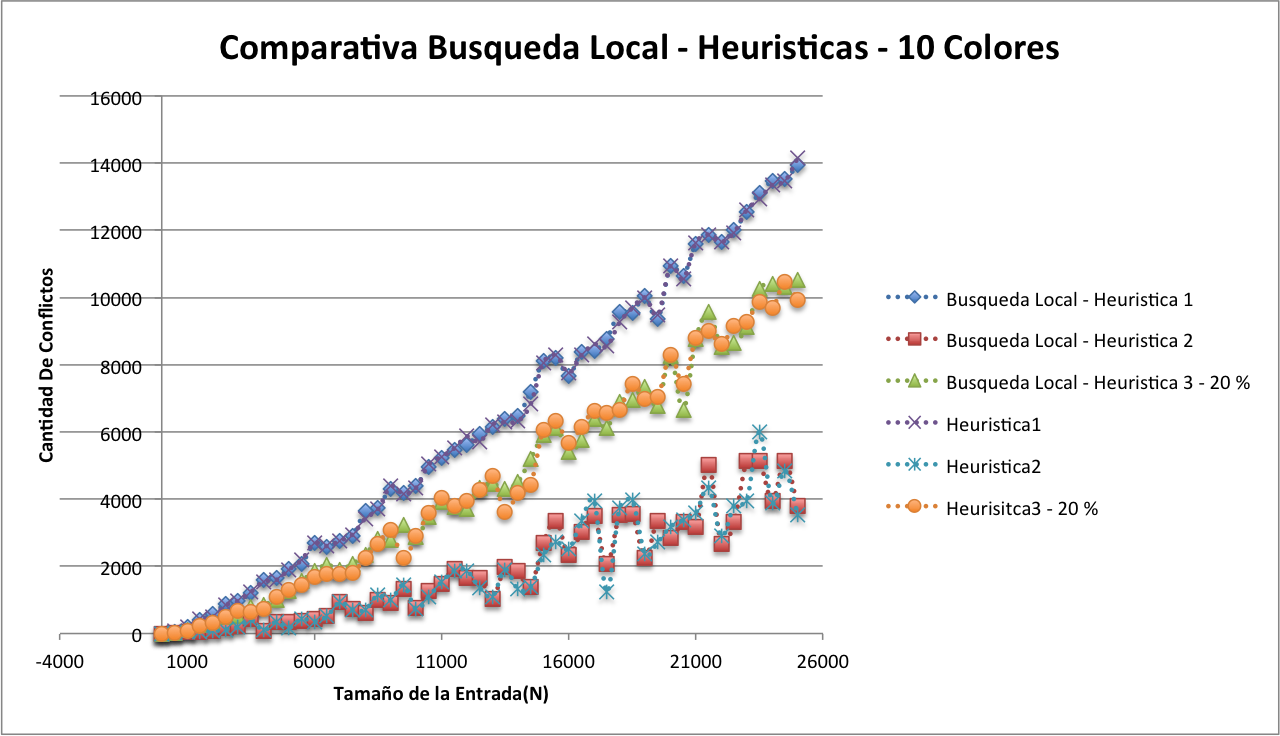
\includegraphics[width=140mm]{ejercicio4/ej4-comparativa-local-heuristicas.png}
\centering
\caption{Comparacion conflictos por heuristica-10 colores}
\label{overflow3}
\end{figure}
Como podiamos imaginar, no existe coloreo valido y vemos que la calidad de nuestro resultado depende mas que nada de la calidad con la cual elegimos nuestra heuristica de arranque. Uno podria suponer que mientras mejor es nuestra subsolucion por donde arrancamos, mejor sera nuestra nuestra solucion final. Sin embargo todavia no sabemos que sucede con la cantidad de iteraciones. Una hipotesis que tenemos es que si arracas con una peor subsolucion, el algortimo tendra la chance de mejorar mayor cantidad de veces y llegar a una mejor solucion que empezando de una buena subsolucion e iterando pocas veces. Luego lo analizaremos para una cantidad de colores mas interesante.\\  

Para analizar el tiempo de ejecucion tenemos que:
\begin{figure}[h!]
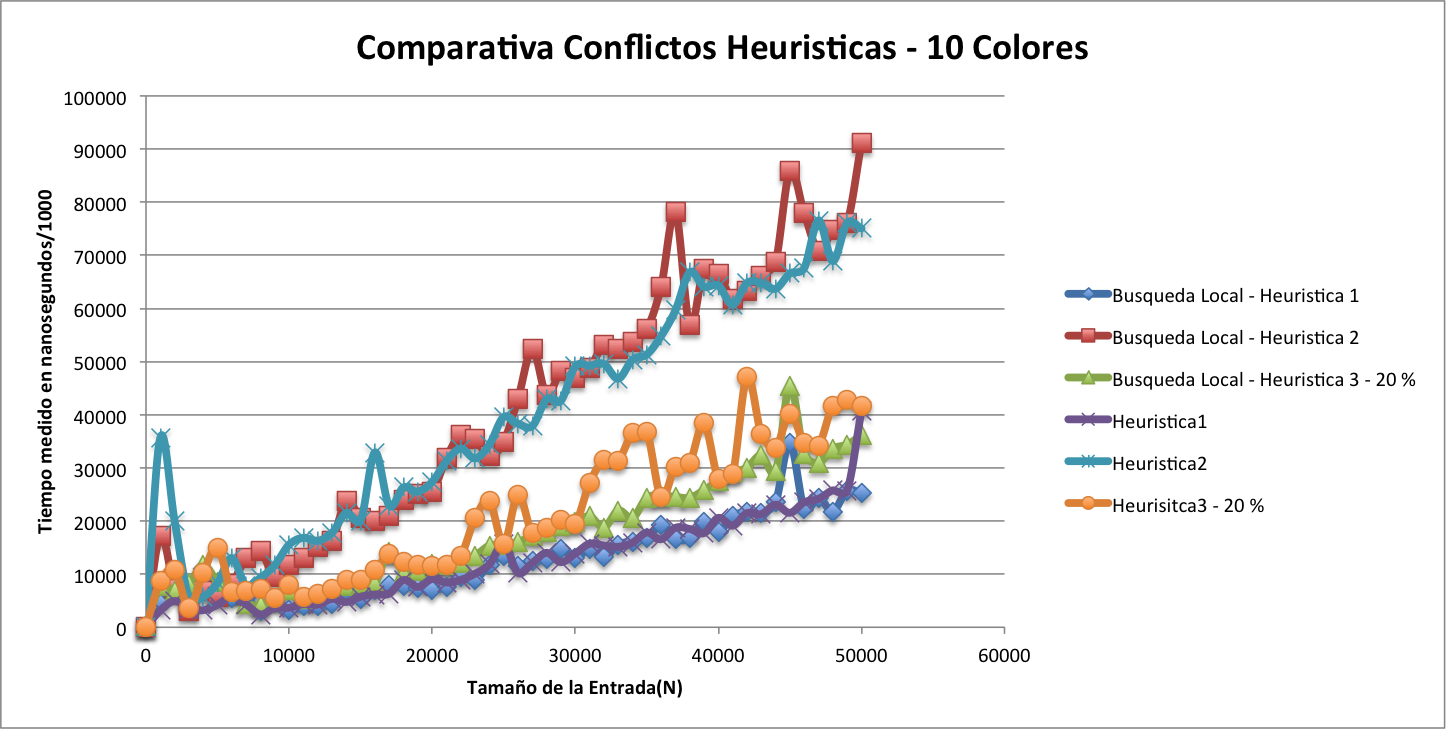
\includegraphics[width=140mm]{ejercicio4/ej4-comparativa-local-heuristicas-10.png}
\centering
\caption{Comparacion Best Vs Worst}
\label{overflow3}
\end{figure}
\pagebreak
La informacion que nos da este grafo es que basicamente el tiempo de ejecucion depende tambien mucho de la heuristica que elijamos al principio. No solo eso sino que nos muestra que nuestra busqueda local nunca podra estar por debajo de la golosa en relacion al tiempo. Ademas el grafico nos muestra que la segunda parte de la suma en en analisis de complejidad (n^2 *MaxCantColores) no es muy relevante y no aporta demasiado al tiempo de ejecucion.\\

Antes de analizar los casos para 500 colores, es trivial que alcanzan para colorear un grafo poco denso de menos de 26k nodos (mayor escala con la cual analizamos el tiempo de ejecucion para 10 colores),\\
Por lotro lado
\begin{figure}[h!]
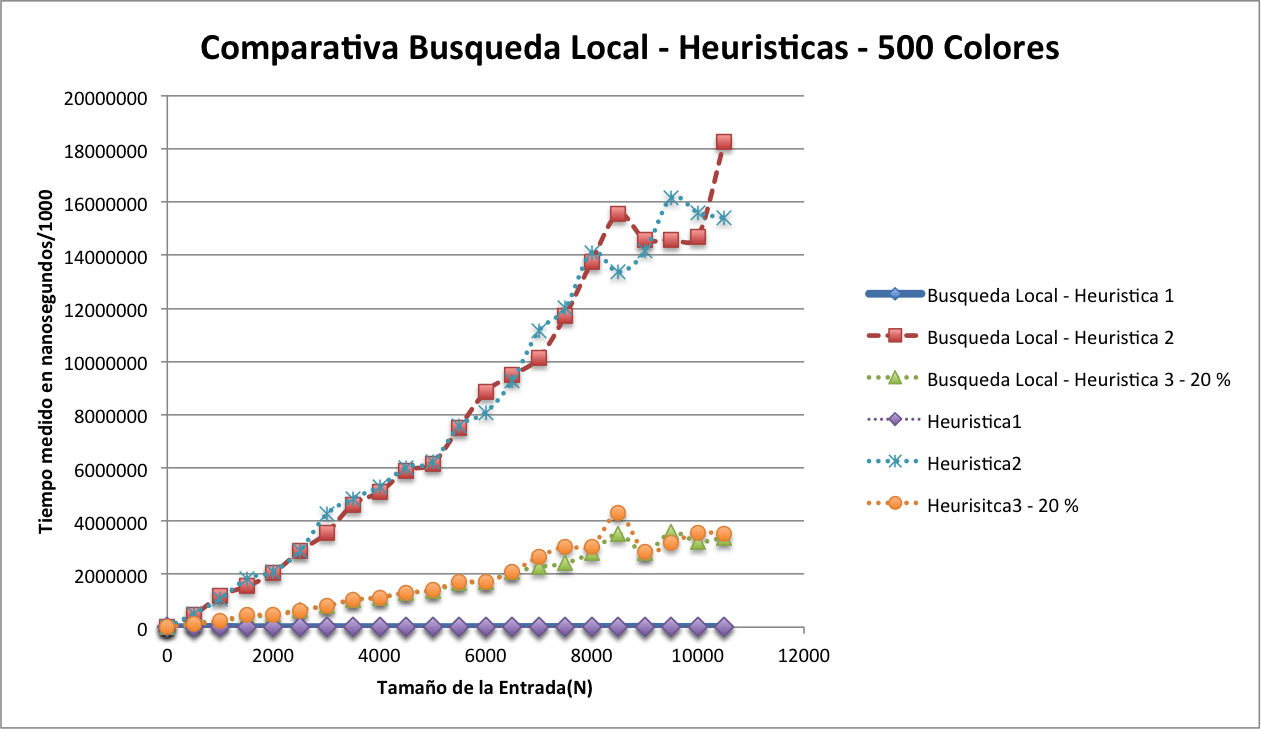
\includegraphics[width=140mm]{ejercicio4/ej4-comparativa-local-heuristicas-500.png}
\centering
\caption{Comparacion Best Vs Worst}
\label{overflow3}
\end{figure}

Para mostrar que realmente la B\'usqueda Local pod\'ia resolver varios conflictos en un grafo, decidimos generar instancias con coloreos muy conflictivos y tratar de mejorarlas con nuestra heur\'istica.
Tomamos grafos de N nodos y los pintamos a todos del mismo color, esto nos crea la mayor cantidad de conflictos posibles para cada uno, variando seg\'un sus conexiones. Luego aplicamos nuestra B\'usqueda local y obtenemos los siguientes resultados

\begin{figure}[h!]
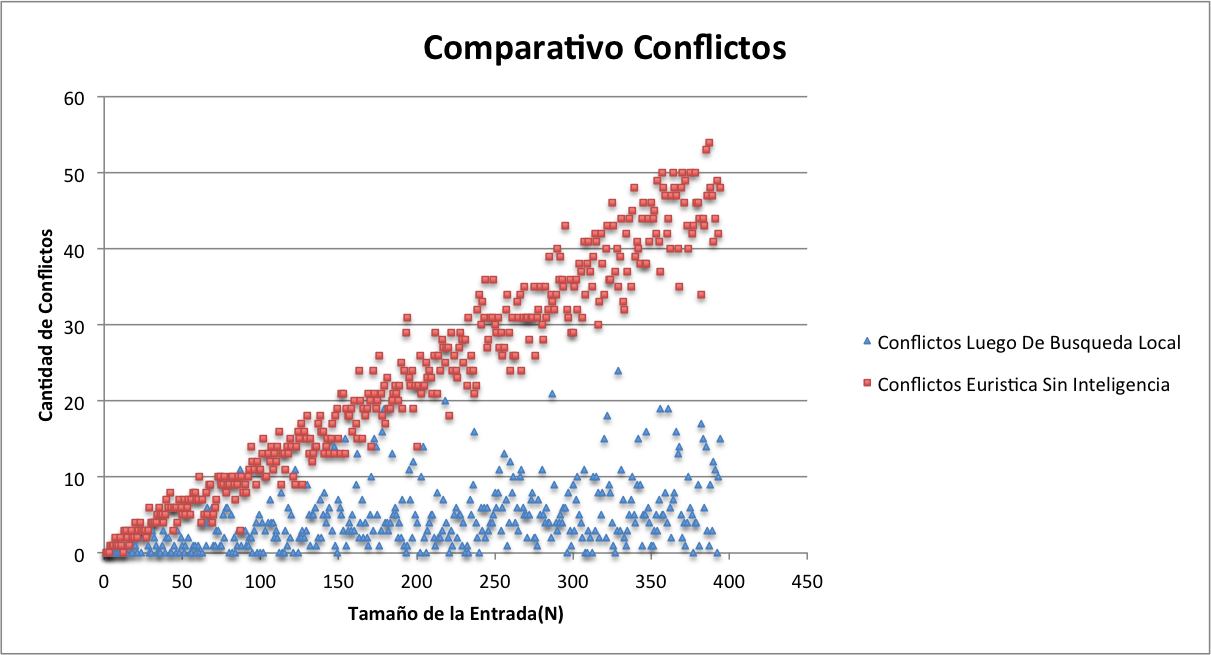
\includegraphics[width=140mm]{ejercicio4/ej4-conflicto}
\centering
\caption{Conflictos reducidos luego de utilizar b\'usqueda lineal.}
\label{overflow3}
\end{figure}
ej4-conflicto

Podemos ver que efectivamente logramos reducir la cantidad de conflictos en gran medida y al ser una b\'usqueda determin\'istica concluimos con que no podr\'iamos encontrar una mejor soluci\'on por este medio. \\

%prueba con una nueva vecindad

Hasta el momento para encontrar alguna modificacion lo que se hacia era probar resolver todos los conflictos individualmente y ver cual mejoro mas la solucion. Como segunda vecindad se intento probar que pasaba si se modificaban todos los nodos al mismo tiempo, esto es si modificar un conflicto redujo los mismos entonces cuando se quiera arreglar el proximo conflicto que tome como base la instancia mejorada previamente.

Para comparar las vecindades se corrierio una instancia del ejercicio3 y sobre esta se corrio el vecindario 1 y 2 por separado y la cantidad de conflictos totales al final de estos fue la siguiente.

\begin{figure}[h!]
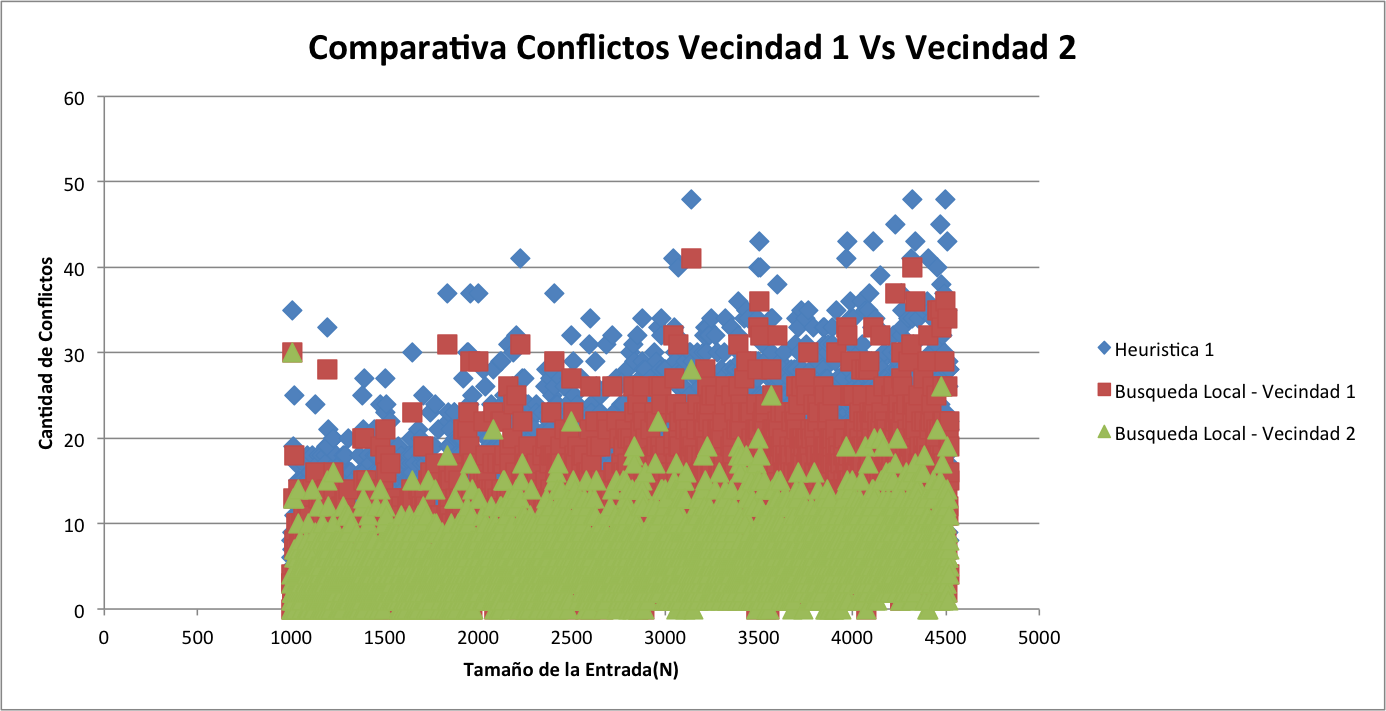
\includegraphics[width=140mm]{ejercicio4/ej4-comparativa-vecindades}
\centering
\caption{Comparaci\'on conflictos ej3 vs vecindarios}
\label{overflow3}
\end{figure}

Se puede observar que arreegla muchos mas conflictos el vecindario 2. Nuestra hipotesis es que al modificar alg\'un conflicto se saca un color de un nodo y se pone otro, esto libera un color y da la posibilidad de que pueda ser utilizado por los nodos vecinos a este y, si el conflicto siguiente es adyacente puede tener la posibilidad de elegir un color diferente a los que podia anteriormente, para algunos casos del vecindario 1 que no tenian mas solucion, este puede dar nuevas posibilidades a los conflictos que esten trabados a poder elegir un color mas.

\pagebreak



\pagebreak
\newpage
\pagebreak
\section{Ejercicio 5}
\subsection{Problema}
Una vez elegidos los mejores valores de configuraci\'on para cada heur\'istica implementada (si fu\'e posible), realizar una \textbf{experimentaci\'on sobre un conjunto nuevo de instancias}  para observar la performance de los m\'etodos comparando nuevamente la calidad de las soluciones obtenidas y los tiempos de ejecuci\'on en funci\'on del tama\~no de entrada. Para los casos que sea posible, comparar tambi\'en los resultados del algoritmo exacto implementado. Presentar todos los resultados obtenidos mediante gr\'aficos adecuados y discutir al respecto de los mismos.
\subsection{Explicaci\'on del problema}

Como los anteriores cuatro ejercicios trabajamos con la misma familia de arboles, buscamos distintas variantes para ver si nuestras heuristicas tiene alguna caracteristica particular segun el tipo de grafo donde la estemos ejecutando. Como vimos anteriormente, para una familia de grafos Kn, la H1 suele tardar menos que la H2 sin embargo la segunda suele conseguir mejores resultados. Ademas vimos que nuestra variante H3 se situa en un punto medio cuando tenemos muchos colores. Cuando tenemos pocos, las tres heuristicas suelen tardar lo mismo. \\
Analizaremos en esta seccion como se comportan los grafos Estrella/Arboles (grafos bipartitos) y que sucede a medida que agregamos aristas a medida que llegamos a obtener nuestro Kn. 
\subsection{Tests y Performance}
Vamos a empezar con un grafo estrella y paso a paso agregaremos 1 arista hasta llegar a un Kn. Lo primero que veremos es que Los grafos estrella se comportan bastante parecidos en relacion a los Kn. vemos en el siguiente grafico que a medida que vamos transformando una estrella en un Kn, el tiempo aumenta de la misma manera.
\pagebreak

\begin{figure}[h!]
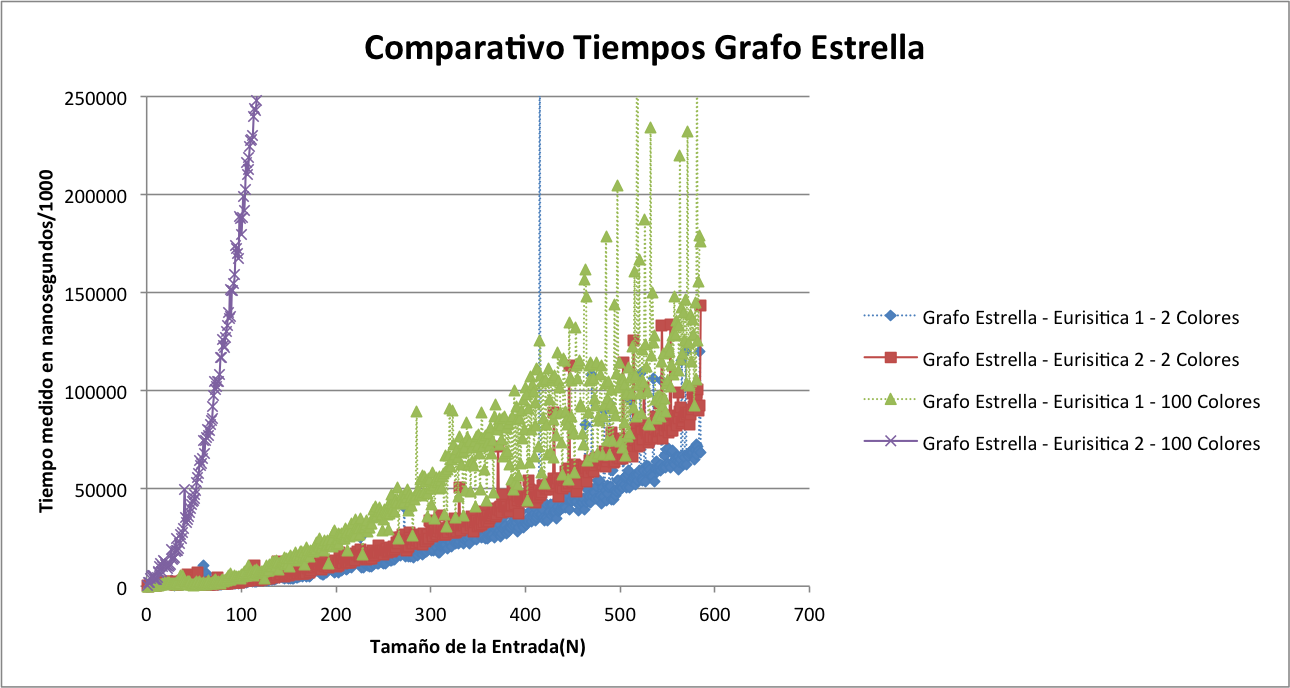
\includegraphics[width=140mm]{ejercicio4/ej5-estrella.png}
\centering
\caption{Cantidad de conflicos HFINAL por solucion}
\label{overflow3}
\end{figure}



Otra cosa que veremos sera como se comporta nuestra solucion de backtrack en comparacion a la "heuristica final". Esta heuristica se basa en nuestro analisis anterior. Miraremos el 20$\%$ de las materias aleatoriamente y si todas tienen mas de 20 colores( es decir que tenemos muchos colores) entonces usaremos la H3. Caso contrario usaremos la H2.


\begin{figure}[h!]
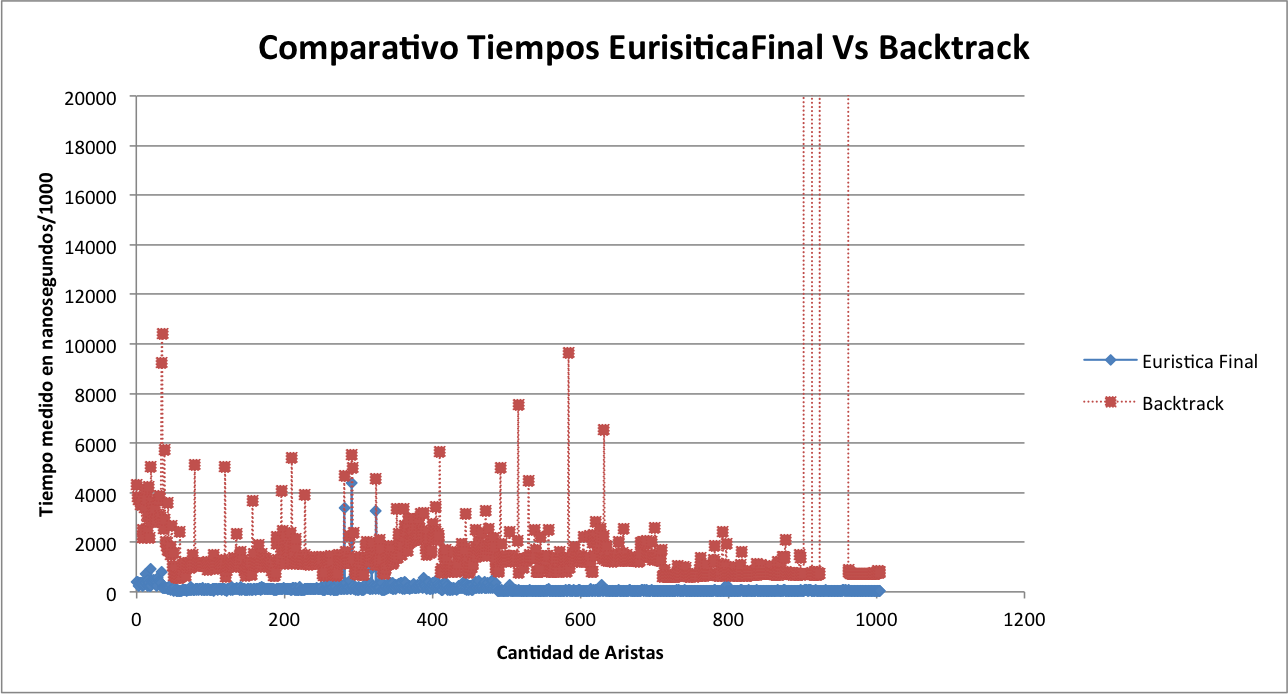
\includegraphics[width=140mm]{ejercicio4/ej5-tiempo-hf-backtrack.png}
\centering
\caption{Comparacion Tiempos estrella HFINAL vs BACKTRACK CON PODAS}
\label{overflow3}
\end{figure}

\pagebreak

En este caso la heuristica final elijio la H2 y lo que muestra el grafico es que si bien el backtrack te asegura la solucion optima, la heruistica final nos dio una cantidad relativamente baja de conflictos y el tiempo se situa extremadamente por debajo. De todos los casos analizados, tuvo el 18,8$\%$ conflictos y ninguno de esos casos tuvo mas de un conflicto. Este porcentaje sale de ver el siguiente grafico: 

\begin{figure}[h!]
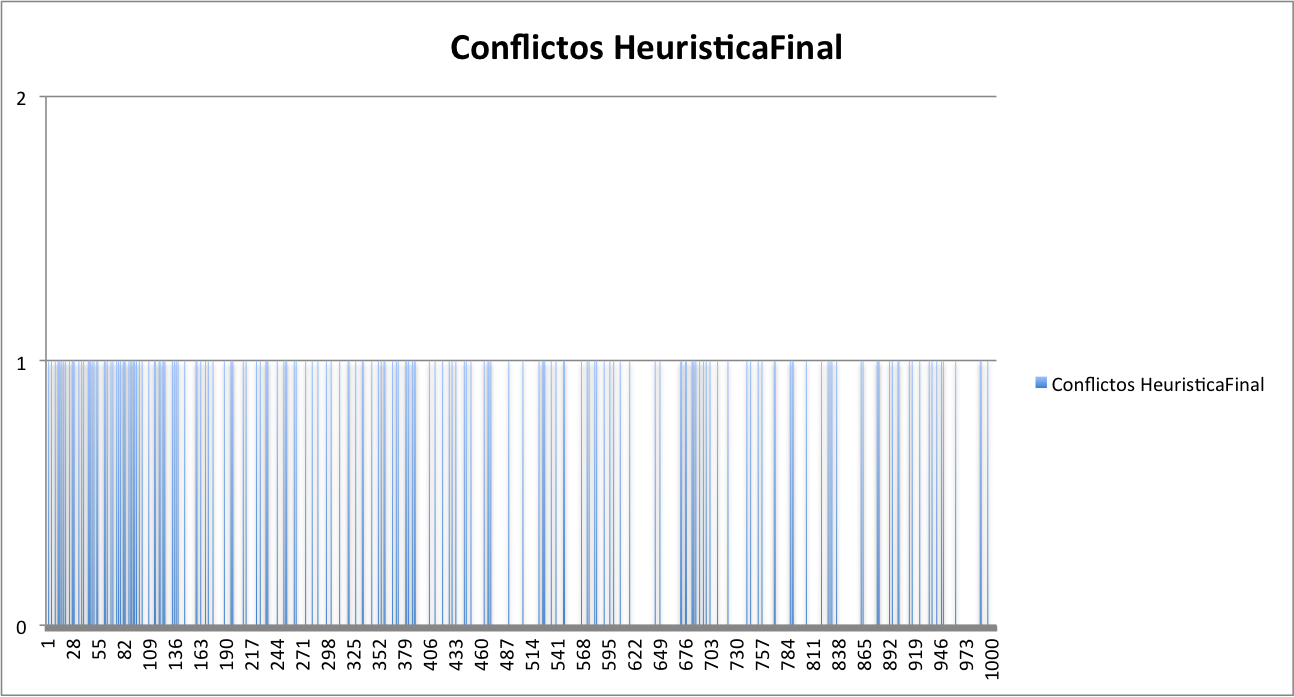
\includegraphics[width=140mm]{ejercicio4/ej5-conflictos.png}
\centering
\caption{Cantidad de conflicos HFINAL por solucion}
\label{overflow3}
\end{figure}
\\
\\
Por ende, si uno prefiere optimalidad, tendra que pagar el costo de corer un algoritmo exacto mientras que si uno tiene un margen de error no tan grande, puede correr una solucion polinomial y tener un resultado aproximado.

Luego decidimos seguir experimentando con nuevas familias de grafos y analizamos los grafos bipartitos completos. Para este realimos nuevos generadores, y nuevos tests para mostrar la diferencia de tiempos entre nuestra mejor euristica y un algoritmo exacto como backtrack.


En el siguiente grafico vemos la comparaci\'on de lo que estabamos proponiendo, y lo que no se observa en el grafico es que los dos algoritmos encuentran una soluci\'on optima sin conflictos.

\begin{figure}[h!]
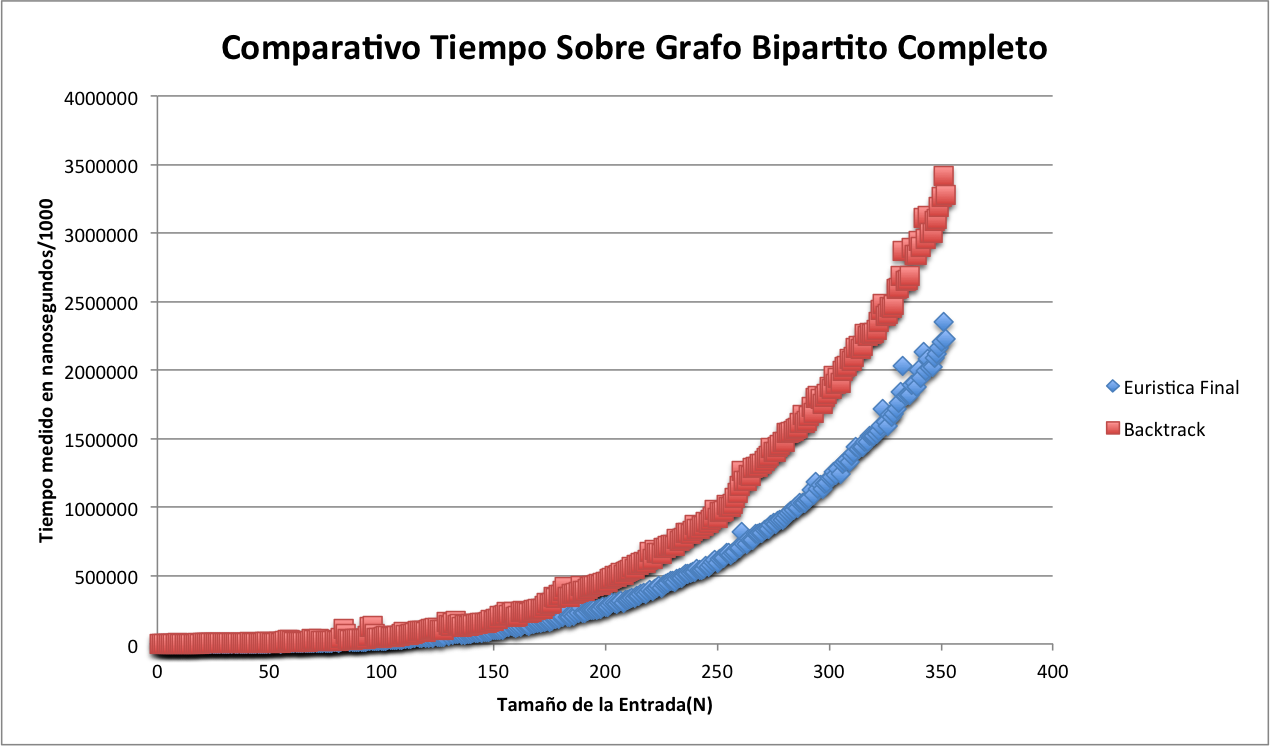
\includegraphics[width=140mm]{ejercicio4/ej5-bipartitoCompleto.png}
\centering
\caption{Cantidad de conflicos HFINAL por solucion}
\label{overflow3}
\end{figure}

Como veniamos probando con muchos grafos estructurados, decidimos empezar a conectar grafos aleatoriamente, intentando evitar familias de grafos conocidas.
Comenzando con 100 nodos desconectados, 8 colores por nodo, fuimos conectando de a 100 aristas en un orden random, para ver como se comportaban los algoritmos. Este test lo podemos plasmar en la siguiente tabla:


\begin{tabular}{| l | l | c | r |}
  \hline
Cantidad aristas & Tiempo Heurisitca & Conflictos Heuristica& Tiempo Backtrack \\ \hline
100 &1133.879 & 36 & 6526.428   \\ \hline
200 &1583.267 & 24 & 8010.119   \\ \hline
300 &1507.946 & 26 & 5874.094   \\ \hline
400 &1770.348 & 21 & 6543.094   \\ \hline
500 &1824.115 & 24 & 5348.103   \\ \hline
600 &2173.457 & 14 & 6424.84   \\ \hline
700 &1397.809 & 19 & 5623.086  \\ \hline
800 &2534.807 & 11 & Tiempo No Medible   \\ \hline
\end{tabular}

\pagebreak
\pagebreak
%\input{modulos/apendice.tex}

\end{document}
